\documentclass[]{article}
\usepackage{lmodern}
\usepackage{amssymb,amsmath}
\usepackage{ifxetex,ifluatex}
\usepackage{fixltx2e} % provides \textsubscript
\ifnum 0\ifxetex 1\fi\ifluatex 1\fi=0 % if pdftex
  \usepackage[T1]{fontenc}
  \usepackage[utf8]{inputenc}
\else % if luatex or xelatex
  \ifxetex
    \usepackage{mathspec}
  \else
    \usepackage{fontspec}
  \fi
  \defaultfontfeatures{Ligatures=TeX,Scale=MatchLowercase}
\fi
% use upquote if available, for straight quotes in verbatim environments
\IfFileExists{upquote.sty}{\usepackage{upquote}}{}
% use microtype if available
\IfFileExists{microtype.sty}{%
\usepackage{microtype}
\UseMicrotypeSet[protrusion]{basicmath} % disable protrusion for tt fonts
}{}
\usepackage[margin=1in]{geometry}
\usepackage{hyperref}
\hypersetup{unicode=true,
            pdftitle={HAMMADDE-ARAMALI İTHALATI, SANAYİ ÜRETİM ENDEKSİ VE İHRACAT MODELİ},
            pdfauthor={Sinem Şenel{[}14080154{]}; Kardelen Kaya{[}15080084{]}; Eray Tekten{[}14080158{]}; Gizem Güzel{[}14080561{]}; Elif Ekinci{[}14080112{]}},
            pdfborder={0 0 0},
            breaklinks=true}
\urlstyle{same}  % don't use monospace font for urls
\usepackage{color}
\usepackage{fancyvrb}
\newcommand{\VerbBar}{|}
\newcommand{\VERB}{\Verb[commandchars=\\\{\}]}
\DefineVerbatimEnvironment{Highlighting}{Verbatim}{commandchars=\\\{\}}
% Add ',fontsize=\small' for more characters per line
\usepackage{framed}
\definecolor{shadecolor}{RGB}{248,248,248}
\newenvironment{Shaded}{\begin{snugshade}}{\end{snugshade}}
\newcommand{\KeywordTok}[1]{\textcolor[rgb]{0.13,0.29,0.53}{\textbf{#1}}}
\newcommand{\DataTypeTok}[1]{\textcolor[rgb]{0.13,0.29,0.53}{#1}}
\newcommand{\DecValTok}[1]{\textcolor[rgb]{0.00,0.00,0.81}{#1}}
\newcommand{\BaseNTok}[1]{\textcolor[rgb]{0.00,0.00,0.81}{#1}}
\newcommand{\FloatTok}[1]{\textcolor[rgb]{0.00,0.00,0.81}{#1}}
\newcommand{\ConstantTok}[1]{\textcolor[rgb]{0.00,0.00,0.00}{#1}}
\newcommand{\CharTok}[1]{\textcolor[rgb]{0.31,0.60,0.02}{#1}}
\newcommand{\SpecialCharTok}[1]{\textcolor[rgb]{0.00,0.00,0.00}{#1}}
\newcommand{\StringTok}[1]{\textcolor[rgb]{0.31,0.60,0.02}{#1}}
\newcommand{\VerbatimStringTok}[1]{\textcolor[rgb]{0.31,0.60,0.02}{#1}}
\newcommand{\SpecialStringTok}[1]{\textcolor[rgb]{0.31,0.60,0.02}{#1}}
\newcommand{\ImportTok}[1]{#1}
\newcommand{\CommentTok}[1]{\textcolor[rgb]{0.56,0.35,0.01}{\textit{#1}}}
\newcommand{\DocumentationTok}[1]{\textcolor[rgb]{0.56,0.35,0.01}{\textbf{\textit{#1}}}}
\newcommand{\AnnotationTok}[1]{\textcolor[rgb]{0.56,0.35,0.01}{\textbf{\textit{#1}}}}
\newcommand{\CommentVarTok}[1]{\textcolor[rgb]{0.56,0.35,0.01}{\textbf{\textit{#1}}}}
\newcommand{\OtherTok}[1]{\textcolor[rgb]{0.56,0.35,0.01}{#1}}
\newcommand{\FunctionTok}[1]{\textcolor[rgb]{0.00,0.00,0.00}{#1}}
\newcommand{\VariableTok}[1]{\textcolor[rgb]{0.00,0.00,0.00}{#1}}
\newcommand{\ControlFlowTok}[1]{\textcolor[rgb]{0.13,0.29,0.53}{\textbf{#1}}}
\newcommand{\OperatorTok}[1]{\textcolor[rgb]{0.81,0.36,0.00}{\textbf{#1}}}
\newcommand{\BuiltInTok}[1]{#1}
\newcommand{\ExtensionTok}[1]{#1}
\newcommand{\PreprocessorTok}[1]{\textcolor[rgb]{0.56,0.35,0.01}{\textit{#1}}}
\newcommand{\AttributeTok}[1]{\textcolor[rgb]{0.77,0.63,0.00}{#1}}
\newcommand{\RegionMarkerTok}[1]{#1}
\newcommand{\InformationTok}[1]{\textcolor[rgb]{0.56,0.35,0.01}{\textbf{\textit{#1}}}}
\newcommand{\WarningTok}[1]{\textcolor[rgb]{0.56,0.35,0.01}{\textbf{\textit{#1}}}}
\newcommand{\AlertTok}[1]{\textcolor[rgb]{0.94,0.16,0.16}{#1}}
\newcommand{\ErrorTok}[1]{\textcolor[rgb]{0.64,0.00,0.00}{\textbf{#1}}}
\newcommand{\NormalTok}[1]{#1}
\usepackage{graphicx,grffile}
\makeatletter
\def\maxwidth{\ifdim\Gin@nat@width>\linewidth\linewidth\else\Gin@nat@width\fi}
\def\maxheight{\ifdim\Gin@nat@height>\textheight\textheight\else\Gin@nat@height\fi}
\makeatother
% Scale images if necessary, so that they will not overflow the page
% margins by default, and it is still possible to overwrite the defaults
% using explicit options in \includegraphics[width, height, ...]{}
\setkeys{Gin}{width=\maxwidth,height=\maxheight,keepaspectratio}
\IfFileExists{parskip.sty}{%
\usepackage{parskip}
}{% else
\setlength{\parindent}{0pt}
\setlength{\parskip}{6pt plus 2pt minus 1pt}
}
\setlength{\emergencystretch}{3em}  % prevent overfull lines
\providecommand{\tightlist}{%
  \setlength{\itemsep}{0pt}\setlength{\parskip}{0pt}}
\setcounter{secnumdepth}{0}
% Redefines (sub)paragraphs to behave more like sections
\ifx\paragraph\undefined\else
\let\oldparagraph\paragraph
\renewcommand{\paragraph}[1]{\oldparagraph{#1}\mbox{}}
\fi
\ifx\subparagraph\undefined\else
\let\oldsubparagraph\subparagraph
\renewcommand{\subparagraph}[1]{\oldsubparagraph{#1}\mbox{}}
\fi

%%% Use protect on footnotes to avoid problems with footnotes in titles
\let\rmarkdownfootnote\footnote%
\def\footnote{\protect\rmarkdownfootnote}

%%% Change title format to be more compact
\usepackage{titling}

% Create subtitle command for use in maketitle
\providecommand{\subtitle}[1]{
  \posttitle{
    \begin{center}\large#1\end{center}
    }
}

\setlength{\droptitle}{-2em}

  \title{HAMMADDE-ARAMALI İTHALATI, SANAYİ ÜRETİM ENDEKSİ VE İHRACAT MODELİ}
    \pretitle{\vspace{\droptitle}\centering\huge}
  \posttitle{\par}
    \author{Sinem Şenel{[}14080154{]} \\ Kardelen Kaya{[}15080084{]} \\ Eray Tekten{[}14080158{]} \\ Gizem Güzel{[}14080561{]} \\ Elif Ekinci{[}14080112{]}}
    \preauthor{\centering\large\emph}
  \postauthor{\par}
      \predate{\centering\large\emph}
  \postdate{\par}
    \date{8 Mayıs 2019}


\begin{document}
\maketitle

\subsection{Özet}\label{ozet}

Çalışmamızda 2007-2019 yılları arasında Türkiye'deki hammadde-ara malı
ithalatı ihracat ve sanayi üretiminin reel efektif döviz kuru, reel
kredi hacmi, OECD ülkelerinin sanayi üretiminden nasıl etkilendiği,
ekonometrik yöntemler kullanılarak analiz edilmiş ve verilen modeller
arasındaki ilişkiler ele alınmıştır. R Studio 3.6.0 programı
kullanılarak modelimizdeki değişken tahminleri ve analizleri
yapılmıştır. Modelde gözlemlenen ekonometrik sorunlar Hausman eşanlılık
testi, içsel bağıntı testi (Breusch-Godfrey LM Testi), değişen varyans
testleri (WHİTE, ARCH) ve RAMSEY RESET testleri ile incelenmiştir.
Çalışmanın sonunda katsayıların ve modelin genel yorumu yapılmıştır.

\subsection{BÖLÜM1: Çalışmanın Amacı ve
Yöntemi}\label{bolum1-calsmann-amac-ve-yontemi}

\subsubsection{1.1 Araştırmanın Amacı}\label{arastrmann-amac}

Bu çalışmada 2007-2019 yılları arasında Türkiye'nin hammadde-ara malı
ithalatı, ihracat ve sanayi üretiminin; reel efektif döviz kuru, reel
kredi hacmi, OECD ülkelerinin sanayi üretiminden nasıl etkilendiği
ekonometrik yöntemler kullanılarak analiz edilmesi amaçlanmıştır.

\subsubsection{1.2 Araştırmanın Yöntemi}\label{arastrmann-yontemi}

Bu çalışmada 3.6.0 R Studio programı kullanılmıştır. Merkez Bankası ve
Dünya Bankası verilerinden yararlanılmıştır. Model 6 değişken ve 145
aylık Yüzde değişimleri içeren veriden oluşmaktadır.Modellerin durağan
ve doğrusal olduğu varsayılmıştır.Analizler bu varsayım üzerinden
yapılacaktır.

\subsubsection{1.3LİTERATÜR}\label{literatur}

Literatürde genel anlamda VAR modelleri, regresyon analizleri, sınır
testi yaklaşımı, Granger nedensellik testleri kullanılarak çalışmalar
yapılmıştır. Elde edilen ampirik bulgulara göre ihracat ve ithalattan
reel efektif döviz kuruna doğru tek yönlü bir nedensellik olduğu
saptanmıştır. GSYİH ile hammadde ve yatırım malı ithalatı arasında çift
yönlü bir ilişki olduğu; fakat GSYİH tüketim malı ve diğer mallar
ithalatı arasında tek yönlü bir ilişki olduğu anlaşılmıştır. Kredi
hacminin ekonomik büyüme üzerindeki etkisi pozitif ve istatistiki olarak
anlamlıdır.

\subsection{BÖLÜM2: Modelimiz}\label{bolum2-modelimiz}

2007:01-2019:01 arasındaki veriler aylık yüzde değişimleri alınarak
kullanılmıştır. Hammadde- aramalı itahalatı 2003 reel baz yılı ile
hesaplanan veriler ile çalışılmıştır.

\subsubsection{2.1 LaTex Formunda
Modeller}\label{latex-formunda-modeller}

\[
mh_t = \beta_0 + \beta_1 y_t + \beta_2 reer_t + \varepsilon_t
\] \[
y_t = \alpha_0 + \alpha_1 mh_t + \alpha_2 rk_t + \alpha_3 reer_t + \varepsilon2_t
\] \[
x_t = \gamma_0 + \gamma_1 ystar_t + \gamma_2 mh_t + \gamma_3 reer_t + \varepsilon3_t
\]

İçsel Değişkenler(Endojenler): Mht=Hammadde-Aramalı İthalatı Yt=Sanayi
Üretim Endeksi(\% değişim) Xt=ihracat(\% değişim)

Dışsal Değişkenler(Eksojenler): reer:Reel efektif döviz kuru rk: Reel
kredi hacmi y*: Yurt dışı sanayi üretim endeksi

\paragraph{2.1.1 Teorik Açıklama}\label{teorik-acklama}

İlk modelde hammadde(ara malı) ithalatının , sanayi üretim endeksinden
ve reel efektif döviz kurundan etkilendiği görülmektedir. Sanayi üretim
endeksi ise hammadde ara malı ithalatından ,reel efektif döviz kurundan
ve reel kredi hacminden etkilenmektedir. Son olarak ihracatın
belirleyenleri ise OECD ülkelerinin sanayi üretim endeksi hammadde ara
malı ithalatı ve reel efektif dövüz kuru olduğu görülmektedir.
Modellerde gecikmeli değişken ve kukla değişken bulunmamaktadır. Sağ
taraf değişkenlerinin sol taraf değişkenlerini kaç birim etkilediğini
katsayı tahminleri kullanılarak yorumlanacaktır.

\subsubsection{2.2 Katsayıların Beklenen
İşaretleri}\label{katsaylarn-beklenen-isaretleri}

Öncelikle katsayıların beklenen işaretleri iktisadi yorumlar
çerçevesinde tahmin edilmiştir.

1Model için; beta1 \textgreater{} 0 (Yt) beta2 \textless{} 0 (reer)

2.Model İçin; alpha1 \textgreater{} 0 (Mh) alpha2 \textgreater{} 0 (rk)

3.Model için; gamma1 \textgreater{}0 (y*) gamma2 \textgreater{}0 (mh)
gamma3 \textgreater{}0 (reer)

\subsubsection{2.3 Ayırt Etme}\label{ayrt-etme}

Yapısal parametrelerin değerlerinin elde edilebilmesi için eşanlı
denklem modellerinin ayrı ayrı belirlenebilir olması gerekir.Modellerin
tahmini için önce sıra ve aşama koşullarına bakılmalıdır.

g*: sistemde bulunan fakat modelde bulunmayan içsel değişken sayısıdır.

k*: sistemde bulunan fakat modelde bulunmayan dışsal değişken sayısıdır.

k:ele alınan modelde önceden belirlenmiş değişken sayısı

g:ele alınan modeldeki endojen değişken sayısı

G:sistemdeki endojen değişken sayısı

K:sistemdeki önceden belirlenmiş değişken sayısı

\(G = mh_t , y_t , x_t\)

\(K = reer_t , rk_t , ystar_t , 1\)

\subsubsection{2.4 Sıra Koşulu}\label{sra-kosulu}

\([\ g^{*} + \ k^{*}] \ge G - 1\)

\begin{enumerate}
\def\labelenumi{\arabic{enumi}.}
\tightlist
\item
  Model
\end{enumerate}

\(k =reer_t , 1\)

\(k^{*} = rk_t , ystar_t\)

\(3 \ge 2\)

fazladan ayırt edilmiştir.

\begin{enumerate}
\def\labelenumi{\arabic{enumi}.}
\setcounter{enumi}{1}
\tightlist
\item
  Model
\end{enumerate}

\(k = rk_t , 1\)

\(k^{*} = ystar _t\)

\(3 \ge 2\)

fazladan ayırt edilmiştir.

\begin{enumerate}
\def\labelenumi{\arabic{enumi}.}
\setcounter{enumi}{2}
\tightlist
\item
  Model
\end{enumerate}

\(k = reer_t , ystar_t\)

\(k^{*} = rk_t 1\)

\(2 \ge 2\)

tam ayırt edilmiştir.

Sıra koşulu yeterli bir koşul olmadığından rank/aşama koşuluna bakarız.

\subsubsection{2.5 Aşama Koşulu}\label{asama-kosulu}

\[\varepsilon_1t = mh_t - \beta_0 + \beta_1 y_t + \beta_2 reer_t\]

\[\varepsilon_2t = y_t - \alpha_0 + \alpha_1 mh_t + \alpha_2 rk_t + alpha_3 reer_t\]

\[\varepsilon_3t= x_t -\gamma_0 + \gamma_1 ystar_t + \gamma_2 mh_t + \gamma_3 reer_t\]

1.denklem için aşama \[\mathbf{S_1} = \left[\begin{array} {rrr}
0 & -\alpha_2 & 0 \\
1 & 0 & -\gamma_1 \\
\end{array}\right]    \begin{vmatrix} S_1 \end{vmatrix} =\begin{vmatrix} 0 & -\alpha_2 \\ 1 & 0 \end{vmatrix} = 0 + \alpha_2 \begin{vmatrix} S_1 \end{vmatrix} \neq 0\]

\(r(S_1)\) : 2\\
\(r(S_1)\) : G-1 tam ayırt edilmiş

2.denklem için aşama \[\mathbf{S_2} = \left[\begin{array} {rrr}
0 & -\beta_2 & 0 \\
1 & -\gamma_3 & -\gamma_1 \\
\end{array}\right]    \begin{vmatrix} S_2 \end{vmatrix} = \begin{vmatrix} 0 & -\beta_2 \\ 1 & -\beta_3 \end{vmatrix} = 0 + \beta_2 \begin{vmatrix} S_2 \end{vmatrix} \neq 0\]

\(r(S_2)\) :2\\
\(r(S_2)\) : G - 1 Tam Ayırt Edilmiş

Bu modelde aşama koşulu yani rank koşulu sağlanmadığı için sıfır
sınırlama yapılmıştır. Kare matrisin determinantının sıfırdan farklı
olması amaçlandığı için reel efektif döviz kuru katsayısı (alpha3) 0
kabul edilmiştir.

3.denklem için aşama \[\mathbf{S_3} = \left[\begin{array} {rrr}
-\beta_1 & 0 \\
1 & -\alpha_2  \\
\end{array}\right]    \begin{vmatrix} S_3 \end{vmatrix} = 0 - (\beta_1 \alpha_2 \begin{vmatrix} S_3 \end{vmatrix} \neq 0\]

\(r(S_3)\) :2\\
\(r(S_3]\) : G - 1 Tam Ayırt Edilmiş

\subsubsection{2.6 İndirgenmiş Formda
Denklemler}\label{indirgenmis-formda-denklemler}

İlk olarak yapısal formdaki denklemlerde endojenler sola, eksojenler
sağa toplanır.

\[
mh_t - \beta_1 y_t = \beta_0 + \beta_2 reer_t + \varepsilon_1t
\]

\[
y_t - \alpha_1 mh_t = \alpha_0 + \alpha_2 rk_t + \varepsilon_2t
\]

\[
x_t - \gamma_2 mh_t = \gamma_0 + \gamma_1 ystar_t + \gamma_3 reer_t + \varepsilon_3t
\]

Ardından matris formunda denklemler şu hale getirilir.

\[
B . Y = \tau . X + \epsilon_t
\]

\[
\mathbf{B.Y} = \left[\begin{array}
{rrr}
1 & -\beta_1 & 0 \\
-\alpha_1 & 1 & 0 \\
-\alpha_2 & 0 & 1
\end{array}\right] 
\]

Modelde Y yalnız bırakılmak için her iki taraf B matrisinin tersi ile
çarpılmıştır.

\[
B^{-1} . B . Y = B^{-1} . \tau . X + B^{-1} . \varepsilon_t
\]

\[
Y = B^{-1} . \tau . X + B^{-1} . \varepsilon_t
\]

\[
\mathbf{B.Y} = \left[\begin{array}
{rrr}
1 & -\beta_1 & 0 \\
-\alpha_1 & 1 & 0 \\
-\alpha_2 & 0 & 1
\end{array}\right] 
\]

\[
\tau . X + \varepsilon_t  = \left[\begin{array}
{rrr}
 \beta_0 + \beta_2\ reer_t + \varepsilon_1t \\
\alpha_0 + \alpha_2\ rk_t + \varepsilon_2t \\
\gamma_0 + \gamma_1\ ystar_t + \gamma_3\ reer_t + \varepsilon_2t \end{array}\right] 
\]

\[
\begin{vmatrix} B \end{vmatrix} = 1 \begin{vmatrix} \ 1 & 0\\ 0 & 1 \end{vmatrix} + -\beta_1 \begin{vmatrix}  -\alpha_1 & 0 \ -\gamma_1 & 1 \end{vmatrix} + 0 \begin{vmatrix} -\alpha_1 & 1 \\ -\gamma_2 & 0 \end{vmatrix} = [1 - \beta_1 \alpha_1 ]
\]

\begin{enumerate}
\def\labelenumi{\arabic{enumi}.}
\tightlist
\item
  model için
\end{enumerate}

\[
\mathbf{mh_t} = \frac{|B_1|}{|B|} = \frac{{\begin{vmatrix} \beta_0 + \beta_2\ reer_t + \varepsilon_1t & -\beta_1 & 0 \\
\alpha_0 + \alpha_2\ rk_t + \varepsilon_2t & 1 & 0 \\
\gamma_ 0 + \gamma_1\ ystar_t + \gamma_3\ reer_t + \varepsilon_3t & 0 & 1
\end{vmatrix}}}{[{1 - \beta_1 . \alpha_1}]}
\]

\[
mh_t = [\beta_0 + \beta_2 reer_t + \varepsilon_1t] . \begin{vmatrix} 1 & 0 \\ 0 & 1 \end{vmatrix} -\beta_1 \begin{vmatrix} \alpha_0 + \alpha_2 rk_t + \varepsilon_2t & 0 \\ \gamma_0 + \gamma_1 ystar_t + \gamma_3 reer_t + \varepsilon_3t & 1 \end{vmatrix} + 0 \begin{vmatrix} \alpha_0 + \alpha_2 rk_t + \varepsilon_2t & 1 \\ \gamma_ 0 + \gamma_1 ystar_t + \gamma_3 reer_t + \varepsilon_3t & 0 \end{vmatrix}
\]

\[
mh_t= \pi_1 + \pi_2 reer_t + \pi_3 rk_t + \pi_4 ystar_t + \ V_1t
\]

\begin{enumerate}
\def\labelenumi{\arabic{enumi}.}
\setcounter{enumi}{1}
\tightlist
\item
  model için
\end{enumerate}

\[
y_t = \frac{|B_2|}{|B|} = \frac{{\begin{vmatrix} 1 & \beta_0 + \beta_2\ reer_t + \varepsilon_1t & 0 \\
-\alpha_1  & \alpha_0 + \alpha_2\ rk_t + \varepsilon_2t & 0 \\
-\gamma_2 & \ gamma_0 + \gamma_1\ ystar_t + \gamma_3\ reer_t + \varepsilon_3t & 1
\end{vmatrix}}}{[{1 - \beta_1 \alpha_1}]}
\]

\[
y_t = 1 \begin{vmatrix} \alpha_0 + \alpha_2\ rk_t + \varepsilon_2t &  0\\
\ gamma_0 + \gamma_1\ ystar_t + \gamma_3\ reer_t + \varepsilon_3t & 1 \end{vmatrix} - [\beta_0 + \beta_2\ reer_t + \varepsilon_1t] \begin{vmatrix} \ -\alpha_1  &  0 \\
 -\gamma_2 & 1 \end{vmatrix} +0 \begin{vmatrix} -\alpha_1 & \alpha_0 + \alpha_2\ rk_t + \varepsilon_2t
\\ -\gamma_2 & \gamma_0 + \gamma_1\ ystar_t + \gamma_3\ reer_t + \varepsilon_3t \end{vmatrix}
\]

\[
y_t= \pi_5 + \pi_6 reer_t + \pi_7 rk_t + \pi_8 ystar_t + \ V_2t
\]

\begin{enumerate}
\def\labelenumi{\arabic{enumi}.}
\setcounter{enumi}{2}
\tightlist
\item
  model için
\end{enumerate}

\[
x_t = \frac{|B_3|}{|B|} = \frac{{\begin{vmatrix} 1 & -\beta_1 & \beta_0 + \beta_2\ reer_t + \varepsilon_1t \\
-\alpha_1\ & 1 &  \alpha_0 + \alpha_2\ rk_t + \varepsilon_2t\\
-\gamma_2\ & 0 & \gamma_0 + \gamma_1\ ystar_t + \gamma_3\ reer_t + \varepsilon_3t
\end{vmatrix}}}{[{1 - \beta_1 . \alpha_1}]}
\]

\[
 x_t = 1 \begin{vmatrix} 1 & \alpha_0 + \alpha_2\ rk_t + \varepsilon_2t \\ 0 & \ gamma_0 + \gamma_1\ ystar_t + \gamma_3\ reer_t + \varepsilon_3t \end{vmatrix} - \\beta_1 \begin{vmatrix} -\alpha_1 & \alpha_0 + \alpha_2\ rk_t + \varepsilon_2t \\ -\gamma_2 & \gamma_0 + \gamma_1\ ystar_t + \gamma_3\ reer_t + \varepsilon_3t \end{vmatrix} + [\beta_0 + \beta_2\ reer_t + \varepsilon_1t] \begin{vmatrix} -\alpha_1 & 1 \\ -\gamma_2 & 0 \end{vmatrix}
\]

\[
 x_t= \pi_9 + \pi_10 reer_t + \pi_11 rk_t + \pi_12 ystar_t + \ V_3t
\]

\begin{Shaded}
\begin{Highlighting}[]
\KeywordTok{library}\NormalTok{(readr)}
\KeywordTok{library}\NormalTok{(tidyverse)}
\end{Highlighting}
\end{Shaded}

\begin{verbatim}
## Registered S3 method overwritten by 'rvest':
##   method            from
##   read_xml.response xml2
\end{verbatim}

\begin{verbatim}
## -- Attaching packages ----------------------------------------------------------------------------------------------- tidyverse 1.2.1 --
\end{verbatim}

\begin{verbatim}
## v ggplot2 3.2.1       v purrr   0.3.2  
## v tibble  2.1.1       v dplyr   0.8.0.1
## v tidyr   0.8.3       v stringr 1.4.0  
## v ggplot2 3.2.1       v forcats 0.4.0
\end{verbatim}

\begin{verbatim}
## -- Conflicts -------------------------------------------------------------------------------------------------- tidyverse_conflicts() --
## x dplyr::filter() masks stats::filter()
## x dplyr::lag()    masks stats::lag()
\end{verbatim}

\begin{Shaded}
\begin{Highlighting}[]
\KeywordTok{library}\NormalTok{(stargazer)}
\end{Highlighting}
\end{Shaded}

\begin{verbatim}
## 
## Please cite as:
\end{verbatim}

\begin{verbatim}
##  Hlavac, Marek (2018). stargazer: Well-Formatted Regression and Summary Statistics Tables.
\end{verbatim}

\begin{verbatim}
##  R package version 5.2.2. https://CRAN.R-project.org/package=stargazer
\end{verbatim}

\begin{Shaded}
\begin{Highlighting}[]
\KeywordTok{library}\NormalTok{(readxl)}
\KeywordTok{library}\NormalTok{(xtable)}
\KeywordTok{library}\NormalTok{(summarytools)}
\end{Highlighting}
\end{Shaded}

\begin{verbatim}
## Registered S3 method overwritten by 'pryr':
##   method      from
##   print.bytes Rcpp
\end{verbatim}

\begin{verbatim}
## 
## Attaching package: 'summarytools'
\end{verbatim}

\begin{verbatim}
## The following objects are masked from 'package:xtable':
## 
##     label, label<-
\end{verbatim}

\begin{verbatim}
## The following object is masked from 'package:tibble':
## 
##     view
\end{verbatim}

\begin{Shaded}
\begin{Highlighting}[]
\KeywordTok{library}\NormalTok{(systemfit)}
\end{Highlighting}
\end{Shaded}

\begin{verbatim}
## Loading required package: Matrix
\end{verbatim}

\begin{verbatim}
## 
## Attaching package: 'Matrix'
\end{verbatim}

\begin{verbatim}
## The following object is masked from 'package:tidyr':
## 
##     expand
\end{verbatim}

\begin{verbatim}
## Loading required package: car
\end{verbatim}

\begin{verbatim}
## Loading required package: carData
\end{verbatim}

\begin{verbatim}
## 
## Attaching package: 'car'
\end{verbatim}

\begin{verbatim}
## The following object is masked from 'package:dplyr':
## 
##     recode
\end{verbatim}

\begin{verbatim}
## The following object is masked from 'package:purrr':
## 
##     some
\end{verbatim}

\begin{verbatim}
## Loading required package: lmtest
\end{verbatim}

\begin{verbatim}
## Loading required package: zoo
\end{verbatim}

\begin{verbatim}
## 
## Attaching package: 'zoo'
\end{verbatim}

\begin{verbatim}
## The following objects are masked from 'package:base':
## 
##     as.Date, as.Date.numeric
\end{verbatim}

\begin{verbatim}
## 
## Please cite the 'systemfit' package as:
## Arne Henningsen and Jeff D. Hamann (2007). systemfit: A Package for Estimating Systems of Simultaneous Equations in R. Journal of Statistical Software 23(4), 1-40. http://www.jstatsoft.org/v23/i04/.
## 
## If you have questions, suggestions, or comments regarding the 'systemfit' package, please use a forum or 'tracker' at systemfit's R-Forge site:
## https://r-forge.r-project.org/projects/systemfit/
\end{verbatim}

\begin{Shaded}
\begin{Highlighting}[]
\KeywordTok{library}\NormalTok{(knitr)}
\KeywordTok{library}\NormalTok{(jtools)}
\KeywordTok{library}\NormalTok{(devtools)}
\KeywordTok{library}\NormalTok{(PoEdata)}
\KeywordTok{library}\NormalTok{(gridExtra)}
\end{Highlighting}
\end{Shaded}

\begin{verbatim}
## 
## Attaching package: 'gridExtra'
\end{verbatim}

\begin{verbatim}
## The following object is masked from 'package:dplyr':
## 
##     combine
\end{verbatim}

\begin{Shaded}
\begin{Highlighting}[]
\KeywordTok{library}\NormalTok{(lmtest)}
\KeywordTok{library}\NormalTok{(broom)}
\KeywordTok{library}\NormalTok{(AER)}
\end{Highlighting}
\end{Shaded}

\begin{verbatim}
## Loading required package: sandwich
\end{verbatim}

\begin{verbatim}
## Loading required package: survival
\end{verbatim}

\begin{verbatim}
## Registered S3 methods overwritten by 'AER':
##   method          from    
##   fitted.survreg  survival
##   nobs.survreg    survival
##   weights.survreg survival
\end{verbatim}

\begin{Shaded}
\begin{Highlighting}[]
\KeywordTok{library}\NormalTok{(car)}
\KeywordTok{library}\NormalTok{(sandwich)}
\KeywordTok{library}\NormalTok{(strucchange)}
\end{Highlighting}
\end{Shaded}

\begin{verbatim}
## 
## Attaching package: 'strucchange'
\end{verbatim}

\begin{verbatim}
## The following object is masked from 'package:stringr':
## 
##     boundary
\end{verbatim}

\begin{Shaded}
\begin{Highlighting}[]
\KeywordTok{library}\NormalTok{(plm)}
\end{Highlighting}
\end{Shaded}

\begin{verbatim}
## Loading required package: Formula
\end{verbatim}

\begin{verbatim}
## 
## Attaching package: 'plm'
\end{verbatim}

\begin{verbatim}
## The following objects are masked from 'package:dplyr':
## 
##     between, lag, lead
\end{verbatim}

\begin{Shaded}
\begin{Highlighting}[]
\NormalTok{veriler <-}\StringTok{ }\KeywordTok{read_csv}\NormalTok{(}\StringTok{"../veriler.csv"}\NormalTok{)}
\end{Highlighting}
\end{Shaded}

\begin{verbatim}
## Parsed with column specification:
## cols(
##   Tarih = col_character(),
##   y = col_double(),
##   reer = col_double(),
##   rk = col_double(),
##   x = col_double(),
##   mh = col_double(),
##   ystar = col_double()
## )
\end{verbatim}

\begin{Shaded}
\begin{Highlighting}[]
\KeywordTok{data}\NormalTok{(veriler)}
\end{Highlighting}
\end{Shaded}

\begin{verbatim}
## Warning in data(veriler): data set 'veriler' not found
\end{verbatim}

\begin{Shaded}
\begin{Highlighting}[]
\KeywordTok{View}\NormalTok{(veriler)}
\KeywordTok{names}\NormalTok{(veriler) <-}\StringTok{ }\KeywordTok{c}\NormalTok{(}\StringTok{"date"}\NormalTok{, }\StringTok{"y"}\NormalTok{, }\StringTok{"reer"}\NormalTok{, }\StringTok{"rk"}\NormalTok{, }\StringTok{"x"}\NormalTok{, }\StringTok{"mh"}\NormalTok{, }\StringTok{"ystar"}\NormalTok{)}
\KeywordTok{summary}\NormalTok{(veriler)}
\end{Highlighting}
\end{Shaded}

\begin{verbatim}
##      date                 y                 reer         
##  Length:145         Min.   :-21.8934   Min.   :-10.9505  
##  Class :character   1st Qu.: -3.7960   1st Qu.: -1.3614  
##  Mode  :character   Median : -0.4114   Median : -0.1834  
##                     Mean   :  0.7249   Mean   : -0.1304  
##                     3rd Qu.:  6.8852   3rd Qu.:  1.1737  
##                     Max.   : 24.1268   Max.   : 10.1356  
##        rk                x                  mh          
##  Min.   :-4.6319   Min.   :-25.0924   Min.   :-9.18760  
##  1st Qu.: 0.7567   1st Qu.: -6.9263   1st Qu.:-1.36510  
##  Median : 1.6768   Median :  0.8057   Median : 0.15850  
##  Mean   : 1.7373   Mean   :  0.8237   Mean   : 0.03152  
##  3rd Qu.: 2.7194   3rd Qu.:  7.1787   3rd Qu.: 1.53850  
##  Max.   :10.4913   Max.   : 30.3564   Max.   : 5.49450  
##      ystar         
##  Min.   :-3.77507  
##  1st Qu.:-0.17603  
##  Median : 0.14629  
##  Mean   : 0.04817  
##  3rd Qu.: 0.47535  
##  Max.   : 1.66670
\end{verbatim}

\subsection{BÖLÜM3:En Küçük Kareler İle
Tahmin}\label{bolum3en-kucuk-kareler-ile-tahmin}

\begin{Shaded}
\begin{Highlighting}[]
\NormalTok{myreg1 <-}\StringTok{ }\KeywordTok{lm}\NormalTok{(mh }\OperatorTok{~}\StringTok{ }\NormalTok{y }\OperatorTok{+}\StringTok{ }\NormalTok{reer, }\DataTypeTok{data =}\NormalTok{ veriler)}
\KeywordTok{summary}\NormalTok{(myreg1)}
\end{Highlighting}
\end{Shaded}

\begin{verbatim}
## 
## Call:
## lm(formula = mh ~ y + reer, data = veriler)
## 
## Residuals:
##     Min      1Q  Median      3Q     Max 
## -9.1831 -1.3377  0.0982  1.4286  5.3168 
## 
## Coefficients:
##              Estimate Std. Error t value Pr(>|t|)
## (Intercept)  0.004841   0.205335   0.024    0.981
## y            0.034944   0.021342   1.637    0.104
## reer        -0.010311   0.079852  -0.129    0.897
## 
## Residual standard error: 2.463 on 142 degrees of freedom
## Multiple R-squared:  0.01881,    Adjusted R-squared:  0.004993 
## F-statistic: 1.361 on 2 and 142 DF,  p-value: 0.2596
\end{verbatim}

\begin{Shaded}
\begin{Highlighting}[]
\NormalTok{myreg2 <-}\StringTok{ }\KeywordTok{lm}\NormalTok{(y }\OperatorTok{~}\StringTok{ }\NormalTok{mh }\OperatorTok{+}\StringTok{ }\NormalTok{rk }\OperatorTok{+}\StringTok{ }\NormalTok{reer, }\DataTypeTok{data =}\NormalTok{ veriler)}
\KeywordTok{summary}\NormalTok{(myreg2)}
\end{Highlighting}
\end{Shaded}

\begin{verbatim}
## 
## Call:
## lm(formula = y ~ mh + rk + reer, data = veriler)
## 
## Residuals:
##      Min       1Q   Median       3Q      Max 
## -20.8032  -5.2037  -0.3154   5.2316  22.9016 
## 
## Coefficients:
##             Estimate Std. Error t value Pr(>|t|)
## (Intercept)  0.07872    1.18960   0.066    0.947
## mh           0.48230    0.33181   1.454    0.148
## rk           0.36061    0.52232   0.690    0.491
## reer        -0.03475    0.36219  -0.096    0.924
## 
## Residual standard error: 9.611 on 141 degrees of freedom
## Multiple R-squared:  0.02388,    Adjusted R-squared:  0.003115 
## F-statistic:  1.15 on 3 and 141 DF,  p-value: 0.3312
\end{verbatim}

\begin{Shaded}
\begin{Highlighting}[]
\NormalTok{myreg3 <-}\StringTok{ }\KeywordTok{lm}\NormalTok{(x }\OperatorTok{~}\StringTok{ }\NormalTok{ystar }\OperatorTok{+}\StringTok{ }\NormalTok{mh }\OperatorTok{+}\StringTok{ }\NormalTok{reer, }\DataTypeTok{data =}\NormalTok{ veriler)}
\KeywordTok{summary}\NormalTok{(myreg3)}
\end{Highlighting}
\end{Shaded}

\begin{verbatim}
## 
## Call:
## lm(formula = x ~ ystar + mh + reer, data = veriler)
## 
## Residuals:
##     Min      1Q  Median      3Q     Max 
## -26.257  -8.076   0.754   6.457  29.822 
## 
## Coefficients:
##             Estimate Std. Error t value Pr(>|t|)   
## (Intercept)   0.7999     0.8763   0.913  0.36292   
## ystar         0.4041     1.2759   0.317  0.75190   
## mh            1.0329     0.3891   2.654  0.00886 **
## reer          0.2157     0.3410   0.633  0.52800   
## ---
## Signif. codes:  0 '***' 0.001 '**' 0.01 '*' 0.05 '.' 0.1 ' ' 1
## 
## Residual standard error: 10.52 on 141 degrees of freedom
## Multiple R-squared:  0.06458,    Adjusted R-squared:  0.04468 
## F-statistic: 3.245 on 3 and 141 DF,  p-value: 0.02391
\end{verbatim}

Modellerimiz tam ve fazladan ayırt edildiği için ekk katsayı tahmin
değerleri tutarsız, T, F ve R2 istatistikleri yukarı sapmalı hesaplanır.
Öncelikle, Modelimizin eşanlılığını test etmemiz gerekiyor.

\begin{Shaded}
\begin{Highlighting}[]
\NormalTok{myregsum1 <-}\StringTok{ }\KeywordTok{summary}\NormalTok{(myreg1)}
\NormalTok{myregsum2 <-}\StringTok{ }\KeywordTok{summary}\NormalTok{(myreg2)}
\NormalTok{myregsum3 <-}\StringTok{ }\KeywordTok{summary}\NormalTok{(myreg3)}

\NormalTok{myregsum1}\OperatorTok{$}\NormalTok{call}
\end{Highlighting}
\end{Shaded}

\begin{verbatim}
## lm(formula = mh ~ y + reer, data = veriler)
\end{verbatim}

\begin{Shaded}
\begin{Highlighting}[]
\NormalTok{myregsum2}\OperatorTok{$}\NormalTok{call}
\end{Highlighting}
\end{Shaded}

\begin{verbatim}
## lm(formula = y ~ mh + rk + reer, data = veriler)
\end{verbatim}

\begin{Shaded}
\begin{Highlighting}[]
\NormalTok{myregsum3}\OperatorTok{$}\NormalTok{call}
\end{Highlighting}
\end{Shaded}

\begin{verbatim}
## lm(formula = x ~ ystar + mh + reer, data = veriler)
\end{verbatim}

\begin{Shaded}
\begin{Highlighting}[]
\NormalTok{myregsum1}\OperatorTok{$}\NormalTok{residuals }\OperatorTok\StringTok{ }\KeywordTok{head}\NormalTok{()}
\end{Highlighting}
\end{Shaded}

\begin{verbatim}
##           1           2           3           4           5           6 
## -2.95441992  0.37993584  1.16010410  2.52681443  2.00254530 -0.01618652
\end{verbatim}

\begin{Shaded}
\begin{Highlighting}[]
\NormalTok{myregsum2}\OperatorTok{$}\NormalTok{residuals }\OperatorTok\StringTok{ }\KeywordTok{head}\NormalTok{()}
\end{Highlighting}
\end{Shaded}

\begin{verbatim}
##             1             2             3             4             5 
## -11.377853553   0.006120355  13.615952766  -7.426603534   6.258482911 
##             6 
##  -1.986243214
\end{verbatim}

\begin{Shaded}
\begin{Highlighting}[]
\NormalTok{myregsum3}\OperatorTok{$}\NormalTok{residuals }\OperatorTok\StringTok{ }\KeywordTok{head}\NormalTok{()}
\end{Highlighting}
\end{Shaded}

\begin{verbatim}
##          1          2          3          4          5          6 
## -22.611622  13.968037  14.505327  -9.902515   7.531497  -4.155329
\end{verbatim}

\begin{Shaded}
\begin{Highlighting}[]
\NormalTok{myregsum1}\OperatorTok{$}\NormalTok{coefficients}
\end{Highlighting}
\end{Shaded}

\begin{verbatim}
##                 Estimate Std. Error     t value  Pr(>|t|)
## (Intercept)  0.004840571 0.20533458  0.02357407 0.9812255
## y            0.034944266 0.02134199  1.63734835 0.1037719
## reer        -0.010311240 0.07985165 -0.12912997 0.8974375
\end{verbatim}

\begin{Shaded}
\begin{Highlighting}[]
\NormalTok{myregsum2}\OperatorTok{$}\NormalTok{coefficients}
\end{Highlighting}
\end{Shaded}

\begin{verbatim}
##                Estimate Std. Error     t value  Pr(>|t|)
## (Intercept)  0.07871699  1.1896047  0.06617071 0.9473356
## mh           0.48230446  0.3318099  1.45355658 0.1482914
## rk           0.36061297  0.5223189  0.69040762 0.4910728
## reer        -0.03475387  0.3621898 -0.09595484 0.9236927
\end{verbatim}

\begin{Shaded}
\begin{Highlighting}[]
\NormalTok{myregsum3}\OperatorTok{$}\NormalTok{coefficients}
\end{Highlighting}
\end{Shaded}

\begin{verbatim}
##              Estimate Std. Error   t value    Pr(>|t|)
## (Intercept) 0.7998630  0.8763009 0.9127720 0.362920520
## ystar       0.4041315  1.2758603 0.3167521 0.751900172
## mh          1.0329395  0.3891470 2.6543685 0.008858902
## reer        0.2157310  0.3410106 0.6326226 0.528004705
\end{verbatim}

\begin{Shaded}
\begin{Highlighting}[]
\NormalTok{myregsum1}\OperatorTok{$}\NormalTok{coefficients[,}\DecValTok{1}\NormalTok{]}
\end{Highlighting}
\end{Shaded}

\begin{verbatim}
##  (Intercept)            y         reer 
##  0.004840571  0.034944266 -0.010311240
\end{verbatim}

\begin{Shaded}
\begin{Highlighting}[]
\NormalTok{myregsum2}\OperatorTok{$}\NormalTok{coefficients[,}\DecValTok{1}\NormalTok{]}
\end{Highlighting}
\end{Shaded}

\begin{verbatim}
## (Intercept)          mh          rk        reer 
##  0.07871699  0.48230446  0.36061297 -0.03475387
\end{verbatim}

\begin{Shaded}
\begin{Highlighting}[]
\NormalTok{myregsum3}\OperatorTok{$}\NormalTok{coefficients[,}\DecValTok{1}\NormalTok{]}
\end{Highlighting}
\end{Shaded}

\begin{verbatim}
## (Intercept)       ystar          mh        reer 
##   0.7998630   0.4041315   1.0329395   0.2157310
\end{verbatim}

\begin{Shaded}
\begin{Highlighting}[]
\NormalTok{myregsum1}\OperatorTok{$}\NormalTok{sigma}
\end{Highlighting}
\end{Shaded}

\begin{verbatim}
## [1] 2.462769
\end{verbatim}

\begin{Shaded}
\begin{Highlighting}[]
\NormalTok{myregsum2}\OperatorTok{$}\NormalTok{sigma}
\end{Highlighting}
\end{Shaded}

\begin{verbatim}
## [1] 9.611364
\end{verbatim}

\begin{Shaded}
\begin{Highlighting}[]
\NormalTok{myregsum3}\OperatorTok{$}\NormalTok{sigma}
\end{Highlighting}
\end{Shaded}

\begin{verbatim}
## [1] 10.51726
\end{verbatim}

\begin{Shaded}
\begin{Highlighting}[]
\NormalTok{myregsum1}\OperatorTok{$}\NormalTok{df}
\end{Highlighting}
\end{Shaded}

\begin{verbatim}
## [1]   3 142   3
\end{verbatim}

\begin{Shaded}
\begin{Highlighting}[]
\NormalTok{myregsum2}\OperatorTok{$}\NormalTok{df}
\end{Highlighting}
\end{Shaded}

\begin{verbatim}
## [1]   4 141   4
\end{verbatim}

\begin{Shaded}
\begin{Highlighting}[]
\NormalTok{myregsum3}\OperatorTok{$}\NormalTok{df}
\end{Highlighting}
\end{Shaded}

\begin{verbatim}
## [1]   4 141   4
\end{verbatim}

\begin{Shaded}
\begin{Highlighting}[]
\NormalTok{myregsum1}\OperatorTok{$}\NormalTok{r.squared}
\end{Highlighting}
\end{Shaded}

\begin{verbatim}
## [1] 0.0188127
\end{verbatim}

\begin{Shaded}
\begin{Highlighting}[]
\NormalTok{myregsum2}\OperatorTok{$}\NormalTok{r.squared}
\end{Highlighting}
\end{Shaded}

\begin{verbatim}
## [1] 0.02388329
\end{verbatim}

\begin{Shaded}
\begin{Highlighting}[]
\NormalTok{myregsum3}\OperatorTok{$}\NormalTok{r.squared}
\end{Highlighting}
\end{Shaded}

\begin{verbatim}
## [1] 0.06458178
\end{verbatim}

\begin{Shaded}
\begin{Highlighting}[]
\NormalTok{myregsum1}\OperatorTok{$}\NormalTok{adj.r.squared}
\end{Highlighting}
\end{Shaded}

\begin{verbatim}
## [1] 0.004993164
\end{verbatim}

\begin{Shaded}
\begin{Highlighting}[]
\NormalTok{myregsum2}\OperatorTok{$}\NormalTok{adj.r.squared}
\end{Highlighting}
\end{Shaded}

\begin{verbatim}
## [1] 0.003114844
\end{verbatim}

\begin{Shaded}
\begin{Highlighting}[]
\NormalTok{myregsum3}\OperatorTok{$}\NormalTok{adj.r.squared}
\end{Highlighting}
\end{Shaded}

\begin{verbatim}
## [1] 0.04467927
\end{verbatim}

\begin{Shaded}
\begin{Highlighting}[]
\NormalTok{myregsum1}\OperatorTok{$}\NormalTok{fstatistic}
\end{Highlighting}
\end{Shaded}

\begin{verbatim}
##      value      numdf      dendf 
##   1.361312   2.000000 142.000000
\end{verbatim}

\begin{Shaded}
\begin{Highlighting}[]
\NormalTok{myregsum2}\OperatorTok{$}\NormalTok{fstatistic}
\end{Highlighting}
\end{Shaded}

\begin{verbatim}
##     value     numdf     dendf 
##   1.14998   3.00000 141.00000
\end{verbatim}

\begin{Shaded}
\begin{Highlighting}[]
\NormalTok{myregsum3}\OperatorTok{$}\NormalTok{fstatistic}
\end{Highlighting}
\end{Shaded}

\begin{verbatim}
##      value      numdf      dendf 
##   3.244905   3.000000 141.000000
\end{verbatim}

\begin{Shaded}
\begin{Highlighting}[]
\NormalTok{myregsum1}\OperatorTok{$}\NormalTok{cov.unscaled}
\end{Highlighting}
\end{Shaded}

\begin{verbatim}
##               (Intercept)             y         reer
## (Intercept)  6.951471e-03 -5.276444e-05 1.277984e-04
## y           -5.276444e-05  7.509694e-05 1.285268e-05
## reer         1.277984e-04  1.285268e-05 1.051285e-03
\end{verbatim}

\begin{Shaded}
\begin{Highlighting}[]
\NormalTok{myregsum2}\OperatorTok{$}\NormalTok{cov.unscaled}
\end{Highlighting}
\end{Shaded}

\begin{verbatim}
##              (Intercept)            mh            rk          reer
## (Intercept)  0.015319172  0.0006291080 -0.0049818233 -0.0016286355
## mh           0.000629108  0.0011918143 -0.0003927958 -0.0001205907
## rk          -0.004981823 -0.0003927958  0.0029532584  0.0010462557
## reer        -0.001628635 -0.0001205907  0.0010462557  0.0014200461
\end{verbatim}

\begin{Shaded}
\begin{Highlighting}[]
\NormalTok{myregsum3}\OperatorTok{$}\NormalTok{cov.unscaled}
\end{Highlighting}
\end{Shaded}

\begin{verbatim}
##               (Intercept)         ystar            mh          reer
## (Intercept)  6.942269e-03 -0.0006290308  4.505558e-05  1.290944e-04
## ystar       -6.290308e-04  0.0147163843 -1.837727e-03  1.681827e-04
## mh           4.505558e-05 -0.0018377271  1.369059e-03 -2.436286e-06
## reer         1.290944e-04  0.0001681827 -2.436286e-06  1.051309e-03
\end{verbatim}

\begin{Shaded}
\begin{Highlighting}[]
\KeywordTok{options}\NormalTok{(}\DataTypeTok{scipen =} \DecValTok{999}\NormalTok{)}
\end{Highlighting}
\end{Shaded}

\subsection{BÖLÜM4:HAUSMAN EŞANLILIK
TESTİ}\label{bolum4hausman-esanlilik-testi}

\begin{Shaded}
\begin{Highlighting}[]
\NormalTok{icsely <-}\StringTok{ }\KeywordTok{lm}\NormalTok{(y }\OperatorTok{~}\StringTok{ }\NormalTok{reer }\OperatorTok{+}\StringTok{ }\NormalTok{rk }\OperatorTok{+}\StringTok{ }\NormalTok{ystar, }\DataTypeTok{data =}\NormalTok{ veriler)}
\NormalTok{what1 <-}\StringTok{ }\KeywordTok{residuals}\NormalTok{(icsely)}
\NormalTok{step11 <-}\StringTok{ }\KeywordTok{lm}\NormalTok{(mh }\OperatorTok{~}\StringTok{ }\NormalTok{y }\OperatorTok{+}\StringTok{ }\NormalTok{reer }\OperatorTok{+}\StringTok{ }\NormalTok{what1, }\DataTypeTok{data =}\NormalTok{ veriler)}
\KeywordTok{summary}\NormalTok{(step11)}
\end{Highlighting}
\end{Shaded}

\begin{verbatim}
## 
## Call:
## lm(formula = mh ~ y + reer + what1, data = veriler)
## 
## Residuals:
##     Min      1Q  Median      3Q     Max 
## -5.9739 -1.5361 -0.0341  1.2248  5.2175 
## 
## Coefficients:
##             Estimate Std. Error t value    Pr(>|t|)    
## (Intercept) -0.57184    0.22016  -2.597      0.0104 *  
## y            0.85570    0.16143   5.301 0.000000435 ***
## reer         0.13016    0.07852   1.658      0.0996 .  
## what1       -0.83312    0.16264  -5.123 0.000000973 ***
## ---
## Signif. codes:  0 '***' 0.001 '**' 0.01 '*' 0.05 '.' 0.1 ' ' 1
## 
## Residual standard error: 2.269 on 141 degrees of freedom
## Multiple R-squared:  0.1728, Adjusted R-squared:  0.1552 
## F-statistic: 9.816 on 3 and 141 DF,  p-value: 0.000006372
\end{verbatim}

\begin{Shaded}
\begin{Highlighting}[]
\NormalTok{icselmh1 <-}\StringTok{ }\KeywordTok{lm}\NormalTok{(mh }\OperatorTok{~}\StringTok{ }\NormalTok{reer }\OperatorTok{+}\StringTok{ }\NormalTok{rk }\OperatorTok{+}\StringTok{ }\NormalTok{ystar, }\DataTypeTok{data =}\NormalTok{ veriler)}
\NormalTok{what2 <-}\StringTok{ }\KeywordTok{residuals}\NormalTok{(icselmh1)}
\NormalTok{step22 <-}\StringTok{ }\KeywordTok{lm}\NormalTok{(y }\OperatorTok{~}\StringTok{ }\NormalTok{mh }\OperatorTok{+}\StringTok{ }\NormalTok{rk }\OperatorTok{+}\StringTok{ }\NormalTok{reer }\OperatorTok{+}\StringTok{ }\NormalTok{what2, }\DataTypeTok{data =}\NormalTok{ veriler)}
\KeywordTok{summary}\NormalTok{(step22)}
\end{Highlighting}
\end{Shaded}

\begin{verbatim}
## 
## Call:
## lm(formula = y ~ mh + rk + reer + what2, data = veriler)
## 
## Residuals:
##      Min       1Q   Median       3Q      Max 
## -20.9681  -5.1076  -0.4396   5.7775  22.6927 
## 
## Coefficients:
##             Estimate Std. Error t value Pr(>|t|)
## (Intercept)  0.32064    1.27110   0.252    0.801
## mh           0.94062    0.89726   1.048    0.296
## rk           0.20956    0.59127   0.354    0.724
## reer        -0.08113    0.37275  -0.218    0.828
## what2       -0.53134    0.96610  -0.550    0.583
## 
## Residual standard error: 9.635 on 140 degrees of freedom
## Multiple R-squared:  0.02599,    Adjusted R-squared:  -0.001841 
## F-statistic: 0.9338 on 4 and 140 DF,  p-value: 0.4463
\end{verbatim}

\begin{Shaded}
\begin{Highlighting}[]
\NormalTok{icselmh2 <-}\StringTok{ }\KeywordTok{lm}\NormalTok{(mh }\OperatorTok{~}\StringTok{ }\NormalTok{reer }\OperatorTok{+}\StringTok{ }\NormalTok{rk }\OperatorTok{+}\StringTok{ }\NormalTok{ystar, }\DataTypeTok{data =}\NormalTok{ veriler)}
\NormalTok{what3 <-}\StringTok{ }\KeywordTok{residuals}\NormalTok{(icselmh2)}
\NormalTok{step33 <-}\StringTok{ }\KeywordTok{lm}\NormalTok{(x }\OperatorTok{~}\StringTok{ }\NormalTok{mh }\OperatorTok{+}\StringTok{ }\NormalTok{ystar }\OperatorTok{+}\StringTok{ }\NormalTok{reer }\OperatorTok{+}\StringTok{ }\NormalTok{what3, }\DataTypeTok{data =}\NormalTok{ veriler)}
\KeywordTok{summary}\NormalTok{(step33)}
\end{Highlighting}
\end{Shaded}

\begin{verbatim}
## 
## Call:
## lm(formula = x ~ mh + ystar + reer + what3, data = veriler)
## 
## Residuals:
##      Min       1Q   Median       3Q      Max 
## -26.0275  -7.6736   0.6633   6.1994  29.8257 
## 
## Coefficients:
##             Estimate Std. Error t value Pr(>|t|)
## (Intercept)   0.8951     0.8879   1.008    0.315
## mh            3.9264     4.0741   0.964    0.337
## ystar        -3.4799     5.5917  -0.622    0.535
## reer          0.2106     0.3417   0.616    0.539
## what3        -2.9202     4.0929  -0.713    0.477
## 
## Residual standard error: 10.54 on 140 degrees of freedom
## Multiple R-squared:  0.06797,    Adjusted R-squared:  0.04134 
## F-statistic: 2.552 on 4 and 140 DF,  p-value: 0.04172
\end{verbatim}

Her modelde içsel olduğunu test edeceğimiz değişkeni indirgenmiş formda
yazdık.indirgenmiş formda yazdığımız içsel olduğunu düşündüğümüz
değişkenlerin hata terimlerini tahmin edip, ana modellere phat1, phat2
ve phat3 olarak yeni bir değişken olarak ekleyip, bu değişkenlerin
katsayılarının anlamlılığını test ettik.

1.model için:

Boş hipotezimiz yt değişkenin birinci modelde eksojen olduğu alternatif
hipotezimiz ise yt nin eksojen olduğu üzerine kurulmuştur.

H0 : y eksojen Ha : y endojen

prob(what1 için); 0.000000973 \textless{} 0.05 olduğu için Ho
reddedilir. y değişkeni mh modelinde içseldir.

2.model için:

H0 : mh eksojen Ha : mh endojen

prob=0.583 \textgreater{} 0.05 Ho kabul edilir. Mh değişkeni, Yt
modelinde dışsaldır.

3.model için:

H0 : mh eksojen Ha : mh endojen

prob=0.477 \textgreater{} 0,05 ise Ho kabul edilir. Mh değişkeni x
denkleminde dışsaldır. İktisadi olarak beklenmeyen sonuçlar ortaya
çıktı. Bu nedenle biz modelimizin tahminine Mh ve Xt'yiiçsel varsayarak
devam edeceğiz.

\subsection{BÖLÜM5:2 Aşamalı En Küçük
Kareler}\label{bolum52-asamal-en-kucuk-kareler}

\begin{Shaded}
\begin{Highlighting}[]
\NormalTok{mh.lm <-}\StringTok{ }\KeywordTok{lm}\NormalTok{(mh }\OperatorTok{~}\StringTok{ }\NormalTok{reer }\OperatorTok{+}\StringTok{ }\NormalTok{rk }\OperatorTok{+}\StringTok{ }\NormalTok{ystar, }\DataTypeTok{data =}\NormalTok{ veriler)}
\KeywordTok{summary}\NormalTok{(mh.lm)}
\end{Highlighting}
\end{Shaded}

\begin{verbatim}
## 
## Call:
## lm(formula = mh ~ reer + rk + ystar, data = veriler)
## 
## Residuals:
##     Min      1Q  Median      3Q     Max 
## -6.7893 -1.4391 -0.0572  1.1311  5.4414 
## 
## Coefficients:
##             Estimate Std. Error t value   Pr(>|t|)    
## (Intercept) -0.27287    0.28253  -0.966      0.336    
## reer         0.05202    0.08564   0.607      0.545    
## rk           0.14447    0.12657   1.141      0.256    
## ystar        1.24948    0.26361   4.740 0.00000517 ***
## ---
## Signif. codes:  0 '***' 0.001 '**' 0.01 '*' 0.05 '.' 0.1 ' ' 1
## 
## Residual standard error: 2.266 on 141 degrees of freedom
## Multiple R-squared:  0.1755, Adjusted R-squared:  0.1579 
## F-statistic:    10 on 3 and 141 DF,  p-value: 0.000005089
\end{verbatim}

\begin{Shaded}
\begin{Highlighting}[]
\NormalTok{veriler}\OperatorTok{$}\NormalTok{phat1 <-}\StringTok{ }\NormalTok{mh.lm}\OperatorTok{$}\NormalTok{fitted.values}
\NormalTok{ikiasamamh.lm <-}\StringTok{ }\KeywordTok{lm}\NormalTok{(mh }\OperatorTok{~}\StringTok{ }\NormalTok{phat1 }\OperatorTok{+}\StringTok{ }\NormalTok{reer, }\DataTypeTok{data =}\NormalTok{ veriler)}
\NormalTok{(ikiaekk1 <-}\StringTok{ }\KeywordTok{summary}\NormalTok{(ikiasamamh.lm))}
\end{Highlighting}
\end{Shaded}

\begin{verbatim}
## 
## Call:
## lm(formula = mh ~ phat1 + reer, data = veriler)
## 
## Residuals:
##     Min      1Q  Median      3Q     Max 
## -6.7893 -1.4391 -0.0572  1.1311  5.4414 
## 
## Coefficients:
##                            Estimate              Std. Error t value
## (Intercept) -0.00000000000000017518  0.18780233588970524083   0.000
## phat1        0.99999999999999966693  0.18205152722752138139   5.493
## reer        -0.00000000000000009357  0.07318291759546773079   0.000
##                Pr(>|t|)    
## (Intercept)           1    
## phat1       0.000000177 ***
## reer                  1    
## ---
## Signif. codes:  0 '***' 0.001 '**' 0.01 '*' 0.05 '.' 0.1 ' ' 1
## 
## Residual standard error: 2.258 on 142 degrees of freedom
## Multiple R-squared:  0.1755, Adjusted R-squared:  0.1639 
## F-statistic: 15.11 on 2 and 142 DF,  p-value: 0.000001122
\end{verbatim}

\begin{Shaded}
\begin{Highlighting}[]
\NormalTok{y.lm <-}\StringTok{ }\KeywordTok{lm}\NormalTok{(y }\OperatorTok{~}\StringTok{ }\NormalTok{reer }\OperatorTok{+}\StringTok{ }\NormalTok{rk }\OperatorTok{+}\StringTok{ }\NormalTok{ystar, }\DataTypeTok{data =}\NormalTok{ veriler)}
\KeywordTok{summary}\NormalTok{(y.lm)}
\end{Highlighting}
\end{Shaded}

\begin{verbatim}
## 
## Call:
## lm(formula = y ~ reer + rk + ystar, data = veriler)
## 
## Residuals:
##      Min       1Q   Median       3Q      Max 
## -23.7468  -4.7361  -0.6832   6.0404  22.5173 
## 
## Coefficients:
##             Estimate Std. Error t value Pr(>|t|)
## (Intercept)  0.06398    1.20285   0.053    0.958
## reer        -0.03219    0.36460  -0.088    0.930
## rk           0.34545    0.53886   0.641    0.523
## ystar        1.17529    1.12232   1.047    0.297
## 
## Residual standard error: 9.646 on 141 degrees of freedom
## Multiple R-squared:  0.0169, Adjusted R-squared:  -0.004014 
## F-statistic: 0.8081 on 3 and 141 DF,  p-value: 0.4914
\end{verbatim}

\begin{Shaded}
\begin{Highlighting}[]
\NormalTok{veriler}\OperatorTok{$}\NormalTok{phat2 <-}\StringTok{ }\NormalTok{y.lm}\OperatorTok{$}\NormalTok{fitted.values}
\NormalTok{ikiasamay.lm <-}\StringTok{ }\KeywordTok{lm}\NormalTok{(y }\OperatorTok{~}\StringTok{ }\NormalTok{phat2 }\OperatorTok{+}\StringTok{ }\NormalTok{rk, }\DataTypeTok{data =}\NormalTok{ veriler)}
\NormalTok{(ikiaekk2 <-}\StringTok{ }\KeywordTok{summary}\NormalTok{(ikiasamay.lm))}
\end{Highlighting}
\end{Shaded}

\begin{verbatim}
## 
## Call:
## lm(formula = y ~ phat2 + rk, data = veriler)
## 
## Residuals:
##      Min       1Q   Median       3Q      Max 
## -23.7468  -4.7361  -0.6832   6.0404  22.5173 
## 
## Coefficients:
##                          Estimate            Std. Error t value Pr(>|t|)
## (Intercept) -0.000000000000000295  1.116723221938501931   0.000    1.000
## phat2        0.999999999999996669  0.950912174445740832   1.052    0.295
## rk           0.000000000000001453  0.655096079134790843   0.000    1.000
## 
## Residual standard error: 9.612 on 142 degrees of freedom
## Multiple R-squared:  0.0169, Adjusted R-squared:  0.003056 
## F-statistic: 1.221 on 2 and 142 DF,  p-value: 0.2981
\end{verbatim}

\begin{Shaded}
\begin{Highlighting}[]
\NormalTok{x.lm <-}\StringTok{ }\KeywordTok{lm}\NormalTok{(x }\OperatorTok{~}\StringTok{ }\NormalTok{reer }\OperatorTok{+}\StringTok{ }\NormalTok{rk }\OperatorTok{+}\StringTok{ }\NormalTok{ystar, }\DataTypeTok{data =}\NormalTok{ veriler)}
\KeywordTok{summary}\NormalTok{(x.lm)}
\end{Highlighting}
\end{Shaded}

\begin{verbatim}
## 
## Call:
## lm(formula = x ~ reer + rk + ystar, data = veriler)
## 
## Residuals:
##      Min       1Q   Median       3Q      Max 
## -25.4756  -8.3593   0.3951   6.2396  30.2634 
## 
## Coefficients:
##             Estimate Std. Error t value Pr(>|t|)
## (Intercept)  -0.1763     1.3397  -0.132    0.895
## reer          0.4149     0.4061   1.022    0.309
## rk            0.5672     0.6002   0.945    0.346
## ystar         1.4261     1.2500   1.141    0.256
## 
## Residual standard error: 10.74 on 141 degrees of freedom
## Multiple R-squared:  0.02402,    Adjusted R-squared:  0.003258 
## F-statistic: 1.157 on 3 and 141 DF,  p-value: 0.3285
\end{verbatim}

\begin{Shaded}
\begin{Highlighting}[]
\NormalTok{veriler}\OperatorTok{$}\NormalTok{phat3 <-}\StringTok{ }\NormalTok{x.lm}\OperatorTok{$}\NormalTok{fitted.values}
\NormalTok{ikiasamax.lm <-}\StringTok{ }\KeywordTok{lm}\NormalTok{(x }\OperatorTok{~}\StringTok{ }\NormalTok{phat3 }\OperatorTok{+}\StringTok{ }\NormalTok{ystar }\OperatorTok{+}\StringTok{ }\NormalTok{reer, }\DataTypeTok{data =}\NormalTok{ veriler)}
\NormalTok{(ikiaekk3 <-}\StringTok{ }\KeywordTok{summary}\NormalTok{(ikiasamax.lm))}
\end{Highlighting}
\end{Shaded}

\begin{verbatim}
## 
## Call:
## lm(formula = x ~ phat3 + ystar + reer, data = veriler)
## 
## Residuals:
##      Min       1Q   Median       3Q      Max 
## -25.4756  -8.3593   0.3951   6.2396  30.2634 
## 
## Coefficients:
##                          Estimate            Std. Error t value Pr(>|t|)
## (Intercept) 0.0000000000000030979 1.2073142213940839529   0.000    1.000
## phat3       0.9999999999999966693 1.0580088929872228931   0.945    0.346
## ystar       0.0000000000000057681 2.2367448092422641537   0.000    1.000
## reer        0.0000000000000007249 0.4175132150008312726   0.000    1.000
## 
## Residual standard error: 10.74 on 141 degrees of freedom
## Multiple R-squared:  0.02402,    Adjusted R-squared:  0.003258 
## F-statistic: 1.157 on 3 and 141 DF,  p-value: 0.3285
\end{verbatim}

İKi aşamalı ekk değerlerini tahmin edebilmek için, denklemlerde içsel
oldğu halde sağ tarafta bulanan değişkenler indirgenmiş formda ekk ile
tahmin edilip, bulunan değerleri ana modellere(yapısal formdaki) tahmin
şeklinde eklenip, bu modellerde 2 aşamalı ekk yöntemi ile katsayı
değerleri tahmin edilmiştir.2AEKK yapılabilmesi için tam veya aşırı
ayırt edilmiş olması gerekir.Küçük örneklemlerde dikkatli
olunmalıdır.2AEKK sonuçları tutarlıdır fakat bu sonuçlar her zaman
sapmazsızlık ve minimum varyans özelliğini sağlayamazlar.

\begin{enumerate}
\def\labelenumi{\arabic{enumi}.}
\tightlist
\item
  modelde içsel olduğunu düşündüğümüz y değişkeninin tahmin değeri phat1
  olarak tanımlanmış ve mh denklemine eklenmiştir. Daha sonra mh
  denklemine 2 aşamalı en küçük kareler yöntemi uygulanmıştır.Bu işlem
  her modele ayrı ayrı uygulanmıştır. iki aşamalı ekk ile yapılan
  katsayı tahmin değerlerinde ekk ile yapılan tahminlere göre R2
  değerleri daha açıklayıcı çıksa da modellerde ibs ve dvs testleri
  henüz yapılmadığı için tahminlerin tutarsız olduğundan
  şüplenilmektedir.
\end{enumerate}

\subsubsection{BÖLÜM 6: SORUNLARIN
TESPİTİ}\label{bolum-6-sorunlarin-tespiti}

\subsection{6.1 İçsel Bağıntı Sorunu}\label{icsel-bagnt-sorunu}

Otokorelasyon sorunu, hata terimlerinin ardışık olarak birbiriyle
ilişkili olması durumudur. İçsel bağıntı sorunun olması katsayı Ekk
tahminlerinin sapmalı olması olmasına sebep olur. Model asimtotik
etkinlik özelliği kaybolur. Modelimizde aylık veriler kullandığımız için
12. dereceden ibs varlığını test ettik. bunun için de en genel bir test
olan 5 aşamalı bg-lm testini kullandık. bu test, model 2 aşamalı ekk ile
tahmin edildikten sonra, hata teriminin tahminin indirgenmiş formda
yazılıp, tekrar ekk ile tahmin edilmesi sonucunda çıkan tahmin değerinin
`'p'' gecikme sayısı olmak üzere p katsayısı ile çarpılarak modele
eklenmesiyle bulunur. en sonda elde edilen genişletilmiş modelin yeni
hata terimi 2 aşamalı ekk ile tahmin edilip indirgenmiş formda
yazılır.Boş hipotez rho değerinin sıfıra eşit olması ve 12. sıradan IBS
olmadığı anlamına gelir.Alternatif hipotez ise rho değerinin sıfıra eşit
olmadığı ve 12. sıradan içsel bağıntı sorununun olduğu durumu gösterir
n(R2y1-r2y2) değerinin hesaplanan kikare değerinden büyük çıkmasıyla boş
hipotez reddedilir. bu durum için boş hipotez gecikme sayısı olan p
değerinin 0 olduğudur., yani ibs olmadığıdır.

\begin{Shaded}
\begin{Highlighting}[]
\KeywordTok{bgtest}\NormalTok{(ikiaekk1, }\DataTypeTok{order =} \DecValTok{12}\NormalTok{, }\DataTypeTok{data =}\NormalTok{ veriler)}
\end{Highlighting}
\end{Shaded}

\begin{verbatim}
## 
##  Breusch-Godfrey test for serial correlation of order up to 12
## 
## data:  ikiaekk1
## LM test = 34.674, df = 12, p-value = 0.0005277
\end{verbatim}

\begin{Shaded}
\begin{Highlighting}[]
\KeywordTok{bgtest}\NormalTok{(ikiaekk2, }\DataTypeTok{order =} \DecValTok{12}\NormalTok{, }\DataTypeTok{data =}\NormalTok{ veriler)}
\end{Highlighting}
\end{Shaded}

\begin{verbatim}
## 
##  Breusch-Godfrey test for serial correlation of order up to 12
## 
## data:  ikiaekk2
## LM test = 105.75, df = 12, p-value < 0.00000000000000022
\end{verbatim}

\begin{Shaded}
\begin{Highlighting}[]
\KeywordTok{bgtest}\NormalTok{(ikiaekk3, }\DataTypeTok{order =} \DecValTok{12}\NormalTok{, }\DataTypeTok{data =}\NormalTok{ veriler)}
\end{Highlighting}
\end{Shaded}

\begin{verbatim}
## 
##  Breusch-Godfrey test for serial correlation of order up to 12
## 
## data:  ikiaekk3
## LM test = 66.164, df = 12, p-value = 0.00000000166
\end{verbatim}

3 modelde de 12. sıradan içsel bağıntı sorunu bulunmaktadır. İçsel
bağıntı sorunun çözümü için C-O dönüştürmesi ya da 2 aşamalı durbin
watson dönüştürmesi yapılabilir.

\subsection{2 aşamalı durbin watson
dönüştürmesi}\label{asamal-durbin-watson-donusturmesi}

Modellerde 12. sıradan içsel bağıntı olduğundan sorunun giderilmesi için
dönüştürme yapılması gerekir.

Modelin 12. sıradan gecikmelileri alınır.

\[mh_{t-12}=\theta_0+\theta_1y_{t-12}+\theta_2reer_{t-12}+\epsilon_{1t-12}\]

\[y_{t-12}=\theta_0+\theta_1mh_{t-12}+\theta_2rk_{t-12}+\epsilon_{2t-12}\]

\[x_{t-12}=\theta_0+\theta_1mh_{t-12}+\theta_2reer_{t-12}+\theta_3rk_{t-12}+\epsilon_{3t-12}\]

Daha sonra \(\rho_12\) katsayısı ile çarpılarak \(mh_t\) modelinden
çıkarılır. Dönüştürmede katsayıların hepsinin aynı anda işleme tabi
tutulması gerekir.

\[
\begin{aligned}
[mh_t-(\rho_12mh_t-{12})] =&\ \theta_0(1-\rho_{12})\\[1.5em]
+&\ \theta_1(y-\rho_{12}y_{t-12})\\[1.5em]
+&\ \theta_2(reer-\rho_{12}reer_{t-12})\\[1.5em]
+&\ \epsilon_{1t} - \rho_{12}\epsilon_{1t-12}
\end{aligned}
\]

\[
\begin{aligned}
[y_t-(\rho_12y_t-{12})] =&\ \theta_0(1-\rho_{12})\\[1.5em]
+&\ \theta_1(mh-\rho_{12}y_{t-12})\\[1.5em]
+&\ \theta_2(rk-\rho_{12}rk_{t-12})\\[1.5em]
+&\ \epsilon_{2t} - \rho_{12}\epsilon_{2t-12}
\end{aligned}
\]

\[
\begin{aligned}
[x_t-(\rho_12x_t-{12})] =&\ \theta_0(1-\rho_{12})\\[1.5em]
+&\ \theta_1(mh-\rho_{12}mh_{t-12})\\[1.5em]
+&\ \theta_2(reer-\rho_{12}reer_{t-12})\\[1.5em]
+&\ \theta_3(rk-\rho_{12}rk_{t-12})\\[1.5em]
+&\ \epsilon_{3t} - \rho_{12}\epsilon_{3t-12}
\end{aligned}
\]

Bu model 2 aşamalı EKK yöntemiyle tahmin edilir ve \(\rho\)
katsayılarının tahmin değerlerine ulaşılır. \(\hat.\rho\) değerleri ile
değişkenlerin gecikmelileri çarpılır. Buradan da değişkenlerin yıldızlı
hallerine ulaşılır ve değikenlerin yıldızlı halleriyle yeni bir model
oluşturulur. Bu yeni oluşturulan model EKK ile tahmin edilerek sorunun
giderilip giderilmediği yeniden test edilir.

\begin{Shaded}
\begin{Highlighting}[]
\NormalTok{yt <-}\StringTok{ }\KeywordTok{lm}\NormalTok{(y }\OperatorTok{~}\StringTok{ }\NormalTok{reer }\OperatorTok{+}\StringTok{ }\NormalTok{rk }\OperatorTok{+}\StringTok{ }\NormalTok{ystar, }\DataTypeTok{data =}\NormalTok{ veriler)}
\KeywordTok{summary}\NormalTok{(ikiaekk1)}
\end{Highlighting}
\end{Shaded}

\begin{verbatim}
##               Length Class  Mode   
## call            3    -none- call   
## terms           3    terms  call   
## residuals     145    -none- numeric
## coefficients   12    -none- numeric
## aliased         3    -none- logical
## sigma           1    -none- numeric
## df              3    -none- numeric
## r.squared       1    -none- numeric
## adj.r.squared   1    -none- numeric
## fstatistic      3    -none- numeric
## cov.unscaled    9    -none- numeric
\end{verbatim}

\begin{Shaded}
\begin{Highlighting}[]
\NormalTok{ytahminmh <-}\StringTok{ }\KeywordTok{predict}\NormalTok{(yt)}
\NormalTok{ikiadurbinmh <-}\StringTok{ }\KeywordTok{lm}\NormalTok{(mh }\OperatorTok{~}\StringTok{ }\OperatorTok{+}\StringTok{ }\KeywordTok{lag}\NormalTok{(mh, }\DecValTok{12}\NormalTok{) }\OperatorTok{+}\StringTok{ }\NormalTok{ytahminmh }\OperatorTok{+}\StringTok{ }\KeywordTok{lag}\NormalTok{(y, }\DecValTok{12}\NormalTok{) }\OperatorTok{+}\StringTok{ }\NormalTok{reer }\OperatorTok{+}\StringTok{ }\KeywordTok{lag}\NormalTok{(reer, }\DecValTok{12}\NormalTok{), }\DataTypeTok{data =}\NormalTok{ veriler)}
\KeywordTok{summary}\NormalTok{(ikiadurbinmh)}
\end{Highlighting}
\end{Shaded}

\begin{verbatim}
## Warning in summary.lm(ikiadurbinmh): essentially perfect fit: summary may
## be unreliable
\end{verbatim}

\begin{verbatim}
## 
## Call:
## lm(formula = mh ~ +lag(mh, 12) + ytahminmh + lag(y, 12) + reer + 
##     lag(reer, 12), data = veriler)
## 
## Residuals:
##                    Min                     1Q                 Median 
## -0.0000000000000068301 -0.0000000000000000179  0.0000000000000000608 
##                     3Q                    Max 
##  0.0000000000000001308  0.0000000000000005868 
## 
## Coefficients: (1 not defined because of singularities)
##                               Estimate               Std. Error
## (Intercept)    0.000000000000000009220  0.000000000000000061339
## lag(mh, 12)    0.999999999999999888978  0.000000000000000022921
## ytahminmh     -0.000000000000000015319  0.000000000000000048208
## lag(y, 12)    -0.000000000000000001885  0.000000000000000005417
## reer          -0.000000000000000021037  0.000000000000000021579
## lag(reer, 12)                       NA                       NA
##                             t value            Pr(>|t|)    
## (Intercept)                   0.150               0.881    
## lag(mh, 12)   43628488774396384.000 <0.0000000000000002 ***
## ytahminmh                    -0.318               0.751    
## lag(y, 12)                   -0.348               0.728    
## reer                         -0.975               0.331    
## lag(reer, 12)                    NA                  NA    
## ---
## Signif. codes:  0 '***' 0.001 '**' 0.01 '*' 0.05 '.' 0.1 ' ' 1
## 
## Residual standard error: 0.0000000000000006176 on 140 degrees of freedom
## Multiple R-squared:      1,  Adjusted R-squared:      1 
## F-statistic: 5.752e+32 on 4 and 140 DF,  p-value: < 0.00000000000000022
\end{verbatim}

\begin{Shaded}
\begin{Highlighting}[]
\NormalTok{rho1 <-}\StringTok{ }\KeywordTok{summary}\NormalTok{(ikiadurbinmh)}\OperatorTok{$}\NormalTok{coefficients[}\DecValTok{2}\NormalTok{,}\DecValTok{1}\NormalTok{]}
\end{Highlighting}
\end{Shaded}

\begin{verbatim}
## Warning in summary.lm(ikiadurbinmh): essentially perfect fit: summary may
## be unreliable
\end{verbatim}

\begin{Shaded}
\begin{Highlighting}[]
\NormalTok{ytstar <-}\StringTok{ }\NormalTok{veriler}\OperatorTok{$}\NormalTok{y }\OperatorTok{-}\StringTok{ }\NormalTok{rho1 }\OperatorTok{*}\StringTok{ }\KeywordTok{lag}\NormalTok{(veriler}\OperatorTok{$}\NormalTok{y)}
\NormalTok{mhstar <-}\StringTok{ }\NormalTok{veriler}\OperatorTok{$}\NormalTok{mh }\OperatorTok{-}\StringTok{ }\NormalTok{rho1 }\OperatorTok{*}\StringTok{ }\KeywordTok{lag}\NormalTok{(veriler}\OperatorTok{$}\NormalTok{mh)}
\NormalTok{reerstar <-}\StringTok{ }\NormalTok{veriler}\OperatorTok{$}\NormalTok{reer }\OperatorTok{-}\StringTok{ }\NormalTok{rho1 }\OperatorTok{*}\StringTok{ }\KeywordTok{lag}\NormalTok{(veriler}\OperatorTok{$}\NormalTok{reer)}
\NormalTok{sonmhstar <-}\StringTok{ }\KeywordTok{data.frame}\NormalTok{(}\DataTypeTok{mhstar =}\NormalTok{ mhstar[}\DecValTok{1}\OperatorTok{:}\DecValTok{133}\NormalTok{], }\DataTypeTok{ytstar =}\NormalTok{ ytstar[}\DecValTok{1}\OperatorTok{:}\DecValTok{133}\NormalTok{], }\DataTypeTok{reerstar =}\NormalTok{ reerstar[}\DecValTok{1}\OperatorTok{:}\DecValTok{133}\NormalTok{])}
\NormalTok{ikiadurbinmh2 <-}\StringTok{ }\KeywordTok{lm}\NormalTok{(mhstar }\OperatorTok{~}\StringTok{ }\NormalTok{ytstar }\OperatorTok{+}\StringTok{ }\NormalTok{reerstar, }\DataTypeTok{data =}\NormalTok{ sonmhstar)}
\KeywordTok{summary}\NormalTok{(ikiadurbinmh2)}
\end{Highlighting}
\end{Shaded}

\begin{verbatim}
## 
## Call:
## lm(formula = mhstar ~ ytstar + reerstar, data = sonmhstar)
## 
## Residuals:
##                     Min                      1Q                  Median 
## -0.00000000000000178037 -0.00000000000000022706  0.00000000000000002122 
##                      3Q                     Max 
##  0.00000000000000023237  0.00000000000000089031 
## 
## Coefficients:
##                           Estimate             Std. Error t value Pr(>|t|)
## (Intercept) 0.00000000000000000606 0.00000000000000003718   0.163    0.871
## ytstar      0.02314060759558515812 0.02334873518115738664   0.991    0.323
## reerstar    0.00687591022098067457 0.09720194665556255997   0.071    0.944
## 
## Residual standard error: 0.0000000000000004272 on 130 degrees of freedom
## Multiple R-squared:  0.007512,   Adjusted R-squared:  -0.007757 
## F-statistic: 0.492 on 2 and 130 DF,  p-value: 0.6126
\end{verbatim}

\begin{Shaded}
\begin{Highlighting}[]
\NormalTok{mht <-}\StringTok{ }\KeywordTok{lm}\NormalTok{(mh }\OperatorTok{~}\StringTok{ }\NormalTok{reer }\OperatorTok{+}\StringTok{ }\NormalTok{rk }\OperatorTok{+}\StringTok{ }\NormalTok{ystar, }\DataTypeTok{data =}\NormalTok{ veriler)}
\KeywordTok{summary}\NormalTok{(ikiaekk2)}
\end{Highlighting}
\end{Shaded}

\begin{verbatim}
##               Length Class  Mode   
## call            3    -none- call   
## terms           3    terms  call   
## residuals     145    -none- numeric
## coefficients   12    -none- numeric
## aliased         3    -none- logical
## sigma           1    -none- numeric
## df              3    -none- numeric
## r.squared       1    -none- numeric
## adj.r.squared   1    -none- numeric
## fstatistic      3    -none- numeric
## cov.unscaled    9    -none- numeric
\end{verbatim}

\begin{Shaded}
\begin{Highlighting}[]
\NormalTok{mhtahminy <-}\StringTok{ }\KeywordTok{predict}\NormalTok{(mht)}
\NormalTok{ikiadurbiny <-}\StringTok{ }\KeywordTok{lm}\NormalTok{(y }\OperatorTok{~}\StringTok{ }\OperatorTok{+}\StringTok{ }\KeywordTok{lag}\NormalTok{(y, }\DecValTok{12}\NormalTok{) }\OperatorTok{+}\StringTok{ }\NormalTok{mhtahminy }\OperatorTok{+}\StringTok{ }\KeywordTok{lag}\NormalTok{(mh, }\DecValTok{12}\NormalTok{) }\OperatorTok{+}\StringTok{ }\NormalTok{rk }\OperatorTok{+}\StringTok{ }\KeywordTok{lag}\NormalTok{(rk, }\DecValTok{12}\NormalTok{), }\DataTypeTok{data =}\NormalTok{ veriler)}
\KeywordTok{summary}\NormalTok{(ikiadurbiny)}
\end{Highlighting}
\end{Shaded}

\begin{verbatim}
## Warning in summary.lm(ikiadurbiny): essentially perfect fit: summary may be
## unreliable
\end{verbatim}

\begin{verbatim}
## 
## Call:
## lm(formula = y ~ +lag(y, 12) + mhtahminy + lag(mh, 12) + rk + 
##     lag(rk, 12), data = veriler)
## 
## Residuals:
##                    Min                     1Q                 Median 
## -0.0000000000000209753 -0.0000000000000000601  0.0000000000000001827 
##                     3Q                    Max 
##  0.0000000000000003194  0.0000000000000028779 
## 
## Coefficients: (1 not defined because of singularities)
##                              Estimate                Std. Error
## (Intercept)  0.0000000000000001475184  0.0000000000000002245357
## lag(y, 12)   0.9999999999999997779554  0.0000000000000000162646
## mhtahminy   -0.0000000000000000932009  0.0000000000000001813037
## lag(mh, 12)  0.0000000000000000043358  0.0000000000000000692575
## rk          -0.0000000000000000005951  0.0000000000000000954703
## lag(rk, 12)                        NA                        NA
##                           t value            Pr(>|t|)    
## (Intercept)                 0.657               0.512    
## lag(y, 12)  61483200169849720.000 <0.0000000000000002 ***
## mhtahminy                  -0.514               0.608    
## lag(mh, 12)                 0.063               0.950    
## rk                         -0.006               0.995    
## lag(rk, 12)                    NA                  NA    
## ---
## Signif. codes:  0 '***' 0.001 '**' 0.01 '*' 0.05 '.' 0.1 ' ' 1
## 
## Residual standard error: 0.000000000000001855 on 140 degrees of freedom
## Multiple R-squared:      1,  Adjusted R-squared:      1 
## F-statistic: 9.699e+32 on 4 and 140 DF,  p-value: < 0.00000000000000022
\end{verbatim}

\begin{Shaded}
\begin{Highlighting}[]
\NormalTok{rho2 <-}\StringTok{ }\KeywordTok{summary}\NormalTok{(ikiadurbiny)}\OperatorTok{$}\NormalTok{coefficients[}\DecValTok{2}\NormalTok{,}\DecValTok{1}\NormalTok{]}
\end{Highlighting}
\end{Shaded}

\begin{verbatim}
## Warning in summary.lm(ikiadurbiny): essentially perfect fit: summary may be
## unreliable
\end{verbatim}

\begin{Shaded}
\begin{Highlighting}[]
\NormalTok{ytstar <-}\StringTok{ }\NormalTok{veriler}\OperatorTok{$}\NormalTok{y }\OperatorTok{-}\StringTok{ }\NormalTok{rho2 }\OperatorTok{*}\StringTok{ }\KeywordTok{lag}\NormalTok{(veriler}\OperatorTok{$}\NormalTok{y)}
\NormalTok{mhstar <-}\StringTok{ }\NormalTok{veriler}\OperatorTok{$}\NormalTok{mh }\OperatorTok{-}\StringTok{ }\NormalTok{rho2 }\OperatorTok{*}\StringTok{ }\KeywordTok{lag}\NormalTok{(veriler}\OperatorTok{$}\NormalTok{mh)}
\NormalTok{rkstar <-}\StringTok{ }\NormalTok{veriler}\OperatorTok{$}\NormalTok{rk }\OperatorTok{-}\StringTok{ }\NormalTok{rho2 }\OperatorTok{*}\StringTok{ }\KeywordTok{lag}\NormalTok{(veriler}\OperatorTok{$}\NormalTok{rk)}
\NormalTok{sonystar <-}\StringTok{ }\KeywordTok{data.frame}\NormalTok{(}\DataTypeTok{mhstar =}\NormalTok{ mhstar[}\DecValTok{1}\OperatorTok{:}\DecValTok{133}\NormalTok{], }\DataTypeTok{ytstar =}\NormalTok{ ytstar[}\DecValTok{1}\OperatorTok{:}\DecValTok{133}\NormalTok{], }\DataTypeTok{rkstar =}\NormalTok{ rkstar[}\DecValTok{1}\OperatorTok{:}\DecValTok{133}\NormalTok{])}
\NormalTok{ikiadurbiny2 <-}\StringTok{ }\KeywordTok{lm}\NormalTok{(ytstar }\OperatorTok{~}\StringTok{ }\NormalTok{mhstar }\OperatorTok{+}\StringTok{ }\NormalTok{rkstar, }\DataTypeTok{data =}\NormalTok{ sonystar)}
\KeywordTok{summary}\NormalTok{(ikiadurbiny2)}
\end{Highlighting}
\end{Shaded}

\begin{verbatim}
## 
## Call:
## lm(formula = ytstar ~ mhstar + rkstar, data = sonystar)
## 
## Residuals:
##                    Min                     1Q                 Median 
## -0.0000000000000039220 -0.0000000000000007800 -0.0000000000000000466 
##                     3Q                    Max 
##  0.0000000000000009098  0.0000000000000038507 
## 
## Coefficients:
##                           Estimate             Std. Error t value Pr(>|t|)
## (Intercept) -0.0000000000000003647  0.0000000000000002128  -1.714  0.08898
## mhstar       0.1502741214629869371  0.3272956138403333992   0.459  0.64690
## rkstar       1.5025487106756671984  0.5671935433815145089   2.649  0.00907
##               
## (Intercept) . 
## mhstar        
## rkstar      **
## ---
## Signif. codes:  0 '***' 0.001 '**' 0.01 '*' 0.05 '.' 0.1 ' ' 1
## 
## Residual standard error: 0.000000000000001567 on 130 degrees of freedom
## Multiple R-squared:  0.05831,    Adjusted R-squared:  0.04382 
## F-statistic: 4.025 on 2 and 130 DF,  p-value: 0.02014
\end{verbatim}

\begin{Shaded}
\begin{Highlighting}[]
\NormalTok{mht <-}\StringTok{ }\KeywordTok{lm}\NormalTok{(mh }\OperatorTok{~}\StringTok{ }\NormalTok{reer }\OperatorTok{+}\StringTok{ }\NormalTok{rk }\OperatorTok{+}\StringTok{ }\NormalTok{ystar, }\DataTypeTok{data =}\NormalTok{ veriler)}
\KeywordTok{summary}\NormalTok{(ikiaekk3)}
\end{Highlighting}
\end{Shaded}

\begin{verbatim}
##               Length Class  Mode   
## call            3    -none- call   
## terms           3    terms  call   
## residuals     145    -none- numeric
## coefficients   16    -none- numeric
## aliased         4    -none- logical
## sigma           1    -none- numeric
## df              3    -none- numeric
## r.squared       1    -none- numeric
## adj.r.squared   1    -none- numeric
## fstatistic      3    -none- numeric
## cov.unscaled   16    -none- numeric
\end{verbatim}

\begin{Shaded}
\begin{Highlighting}[]
\NormalTok{mhtahminx <-}\StringTok{ }\KeywordTok{predict}\NormalTok{(mht)}
\NormalTok{ikiadurbinx <-}\StringTok{ }\KeywordTok{lm}\NormalTok{(x }\OperatorTok{~}\StringTok{ }\OperatorTok{+}\StringTok{ }\KeywordTok{lag}\NormalTok{(x, }\DecValTok{12}\NormalTok{) }\OperatorTok{+}\StringTok{ }\NormalTok{mhtahminx }\OperatorTok{+}\StringTok{ }\KeywordTok{lag}\NormalTok{(mh, }\DecValTok{12}\NormalTok{) }\OperatorTok{+}\StringTok{ }\NormalTok{reer }\OperatorTok{+}\StringTok{ }\KeywordTok{lag}\NormalTok{(reer, }\DecValTok{12}\NormalTok{) }\OperatorTok{+}\StringTok{ }\NormalTok{ystar }\OperatorTok{+}\StringTok{ }\KeywordTok{lag}\NormalTok{(ystar, }\DecValTok{12}\NormalTok{), }\DataTypeTok{data =}\NormalTok{ veriler)}
\KeywordTok{summary}\NormalTok{(ikiadurbinx)}
\end{Highlighting}
\end{Shaded}

\begin{verbatim}
## Warning in summary.lm(ikiadurbinx): essentially perfect fit: summary may be
## unreliable
\end{verbatim}

\begin{verbatim}
## 
## Call:
## lm(formula = x ~ +lag(x, 12) + mhtahminx + lag(mh, 12) + reer + 
##     lag(reer, 12) + ystar + lag(ystar, 12), data = veriler)
## 
## Residuals:
##                    Min                     1Q                 Median 
## -0.0000000000000039583 -0.0000000000000004369 -0.0000000000000001342 
##                     3Q                    Max 
##  0.0000000000000002384  0.0000000000000251676 
## 
## Coefficients: (2 not defined because of singularities)
##                               Estimate              Std. Error
## (Intercept)    -0.00000000000000014752  0.00000000000000019200
## lag(x, 12)      1.00000000000000022204  0.00000000000000001821
## mhtahminx       0.00000000000000102329  0.00000000000000088342
## lag(mh, 12)    -0.00000000000000002377  0.00000000000000008634
## reer            0.00000000000000009076  0.00000000000000007372
## lag(reer, 12)                       NA                      NA
## ystar          -0.00000000000000120615  0.00000000000000120642
## lag(ystar, 12)                      NA                      NA
##                              t value            Pr(>|t|)    
## (Intercept)                   -0.768               0.444    
## lag(x, 12)     54917345087619304.000 <0.0000000000000002 ***
## mhtahminx                      1.158               0.249    
## lag(mh, 12)                   -0.275               0.784    
## reer                           1.231               0.220    
## lag(reer, 12)                     NA                  NA    
## ystar                         -1.000               0.319    
## lag(ystar, 12)                    NA                  NA    
## ---
## Signif. codes:  0 '***' 0.001 '**' 0.01 '*' 0.05 '.' 0.1 ' ' 1
## 
## Residual standard error: 0.00000000000000227 on 139 degrees of freedom
## Multiple R-squared:      1,  Adjusted R-squared:      1 
## F-statistic: 6.472e+32 on 5 and 139 DF,  p-value: < 0.00000000000000022
\end{verbatim}

\begin{Shaded}
\begin{Highlighting}[]
\NormalTok{rho3 <-}\StringTok{ }\KeywordTok{summary}\NormalTok{(ikiadurbinx)}\OperatorTok{$}\NormalTok{coefficients[}\DecValTok{2}\NormalTok{,}\DecValTok{1}\NormalTok{]}
\end{Highlighting}
\end{Shaded}

\begin{verbatim}
## Warning in summary.lm(ikiadurbinx): essentially perfect fit: summary may be
## unreliable
\end{verbatim}

\begin{Shaded}
\begin{Highlighting}[]
\NormalTok{ystarstar <-}\StringTok{ }\NormalTok{veriler}\OperatorTok{$}\NormalTok{ystar }\OperatorTok{-}\StringTok{ }\NormalTok{rho3 }\OperatorTok{*}\StringTok{ }\KeywordTok{lag}\NormalTok{(veriler}\OperatorTok{$}\NormalTok{ystar)}
\NormalTok{mhstar <-}\StringTok{ }\NormalTok{veriler}\OperatorTok{$}\NormalTok{mh }\OperatorTok{-}\StringTok{ }\NormalTok{rho3 }\OperatorTok{*}\StringTok{ }\KeywordTok{lag}\NormalTok{(veriler}\OperatorTok{$}\NormalTok{mh)}
\NormalTok{xstar <-}\StringTok{ }\NormalTok{veriler}\OperatorTok{$}\NormalTok{x }\OperatorTok{-}\StringTok{ }\NormalTok{rho3 }\OperatorTok{*}\StringTok{ }\KeywordTok{lag}\NormalTok{(veriler}\OperatorTok{$}\NormalTok{x)}
\NormalTok{reerstar <-}\StringTok{ }\NormalTok{veriler}\OperatorTok{$}\NormalTok{reer }\OperatorTok{-}\StringTok{ }\NormalTok{rho3 }\OperatorTok{*}\StringTok{ }\KeywordTok{lag}\NormalTok{(veriler}\OperatorTok{$}\NormalTok{reer)}
\NormalTok{sonxstar <-}\StringTok{ }\KeywordTok{data.frame}\NormalTok{(}\DataTypeTok{mhstar =}\NormalTok{ mhstar[}\DecValTok{1}\OperatorTok{:}\DecValTok{133}\NormalTok{], }\DataTypeTok{xstar =}\NormalTok{ xstar[}\DecValTok{1}\OperatorTok{:}\DecValTok{133}\NormalTok{], }\DataTypeTok{ystarstar =}\NormalTok{ ystarstar[}\DecValTok{1}\OperatorTok{:}\DecValTok{133}\NormalTok{], }\DataTypeTok{reerstar =}\NormalTok{ reerstar[}\DecValTok{1}\OperatorTok{:}\DecValTok{133}\NormalTok{])}
\NormalTok{ikiadurbinx2 <-}\StringTok{ }\KeywordTok{lm}\NormalTok{(xstar }\OperatorTok{~}\StringTok{ }\NormalTok{mhstar }\OperatorTok{+}\StringTok{ }\NormalTok{reerstar }\OperatorTok{+}\StringTok{ }\NormalTok{ystarstar, }\DataTypeTok{data =}\NormalTok{ sonxstar)}
\KeywordTok{summary}\NormalTok{(ikiadurbinx2)}
\end{Highlighting}
\end{Shaded}

\begin{verbatim}
## 
## Call:
## lm(formula = xstar ~ mhstar + reerstar + ystarstar, data = sonxstar)
## 
## Residuals:
##                    Min                     1Q                 Median 
## -0.0000000000000069911 -0.0000000000000013131  0.0000000000000001351 
##                     3Q                    Max 
##  0.0000000000000015147  0.0000000000000063207 
## 
## Coefficients:
##                           Estimate             Std. Error t value Pr(>|t|)
## (Intercept) -0.0000000000000002341  0.0000000000000001980  -1.183   0.2392
## mhstar       1.0758832959310145050  0.4044576142499578530   2.660   0.0088
## reerstar    -0.2894750239719822704  0.4391584048265808615  -0.659   0.5110
## ystarstar   -0.0382368550731230911  1.1941880418464529967  -0.032   0.9745
##               
## (Intercept)   
## mhstar      **
## reerstar      
## ystarstar     
## ---
## Signif. codes:  0 '***' 0.001 '**' 0.01 '*' 0.05 '.' 0.1 ' ' 1
## 
## Residual standard error: 0.000000000000002276 on 129 degrees of freedom
## Multiple R-squared:  0.06481,    Adjusted R-squared:  0.04307 
## F-statistic:  2.98 on 3 and 129 DF,  p-value: 0.0339
\end{verbatim}

\subsection{6.2 Değişen Varyans Sorunu}\label{degisen-varyans-sorunu}

\subsection{white testi}\label{white-testi}

Model 2 aşamalı ekk ile tahmin edilir. Hata teriminin tahminlerinin
kareleri denklemi oluşturulur. Bu denkleme yapısal modeldeki
değişkenler, kareleri, değişkenlerin birbirleri ile çarpımı eklenir.
Oluşturulan model ekk ile tahmin edilir. R2 değeri ya da F istatistiği
ile ana model ve yardımcı modelin rss değerlerinden boş hipotezi kabul
ya da reddeceğimize karar veririz. Hesaplanan değer tablo değerinden
büyükse boş hipotez reddedilir. Boş hipotezimiz yardımcı modelin
değişkenlerinin katsayılarının sıfıra eşit oluğu yani, değişen varyans
sorunu olmamasıdır. ny(R\textsuperscript{2y1-R}2y2) test istatistiği
hesaplanarak X\^{}2(k-1) tablo değeri ile karşılaştırılabilir.K-1 Bize
modelde sabit terim hariç değişken adedini veren serbestlik
derecesidir.Bu testte p-value değerlerine bakarak sonuca ulaştık.

Ho : yardımcı model katsayıları = 0 ha : en az biri sıfır değil

\begin{Shaded}
\begin{Highlighting}[]
\KeywordTok{bptest}\NormalTok{(ikiaekk1, }\OperatorTok{~}\StringTok{ }\NormalTok{y }\OperatorTok{+}\StringTok{ }\KeywordTok{I}\NormalTok{(y}\OperatorTok{^}\DecValTok{2}\NormalTok{) }\OperatorTok{+}\StringTok{ }\NormalTok{reer }\OperatorTok{+}\StringTok{ }\KeywordTok{I}\NormalTok{(reer}\OperatorTok{^}\DecValTok{2}\NormalTok{), }\DataTypeTok{data =}\NormalTok{ veriler)}
\end{Highlighting}
\end{Shaded}

\begin{verbatim}
## 
##  studentized Breusch-Pagan test
## 
## data:  ikiaekk1
## BP = 4.6506, df = 4, p-value = 0.3251
\end{verbatim}

\begin{Shaded}
\begin{Highlighting}[]
\KeywordTok{bptest}\NormalTok{(ikiaekk2, }\OperatorTok{~}\StringTok{ }\NormalTok{mh }\OperatorTok{+}\StringTok{ }\KeywordTok{I}\NormalTok{(mh}\OperatorTok{^}\DecValTok{2}\NormalTok{) }\OperatorTok{+}\StringTok{ }\NormalTok{rk }\OperatorTok{+}\StringTok{ }\KeywordTok{I}\NormalTok{(rk}\OperatorTok{^}\DecValTok{2}\NormalTok{) }\OperatorTok{+}\StringTok{ }\NormalTok{reer, }\DataTypeTok{data =}\NormalTok{ veriler)}
\end{Highlighting}
\end{Shaded}

\begin{verbatim}
## 
##  studentized Breusch-Pagan test
## 
## data:  ikiaekk2
## BP = 10.849, df = 5, p-value = 0.05446
\end{verbatim}

\begin{Shaded}
\begin{Highlighting}[]
\KeywordTok{bptest}\NormalTok{(ikiaekk3, }\OperatorTok{~}\StringTok{ }\NormalTok{ystar }\OperatorTok{+}\StringTok{ }\KeywordTok{I}\NormalTok{(ystar}\OperatorTok{^}\DecValTok{2}\NormalTok{) }\OperatorTok{+}\StringTok{ }\NormalTok{mh }\OperatorTok{+}\StringTok{ }\KeywordTok{I}\NormalTok{(mh}\OperatorTok{^}\DecValTok{2}\NormalTok{) }\OperatorTok{+}\StringTok{ }\NormalTok{reer }\OperatorTok{+}\StringTok{ }\KeywordTok{I}\NormalTok{(reer}\OperatorTok{^}\DecValTok{2}\NormalTok{), }\DataTypeTok{data =}\NormalTok{ veriler)}
\end{Highlighting}
\end{Shaded}

\begin{verbatim}
## 
##  studentized Breusch-Pagan test
## 
## data:  ikiaekk3
## BP = 2.233, df = 6, p-value = 0.8971
\end{verbatim}

3 model için de white formunda dvs yoktur. Zaman serileri ile
çalıştığımız için, white formunda dvs bulmamamız normal bir sonuçtur ve
bakmamız gereken arch formunda dvs'dir.

\subsection{Arch Formunda Değişen Varyans
Testi}\label{arch-formunda-degisen-varyans-testi}

\begin{Shaded}
\begin{Highlighting}[]
\NormalTok{resids1 <-}\StringTok{ }\KeywordTok{resid}\NormalTok{(ikiaekk1)}
\NormalTok{resids11 <-}\StringTok{ }\NormalTok{resids1}\OperatorTok{^}\DecValTok{2}
\NormalTok{auxreg1 <-}\StringTok{ }\KeywordTok{lm}\NormalTok{(resids11 }\OperatorTok{~}\StringTok{ }\KeywordTok{lag}\NormalTok{(resids11, }\DecValTok{12}\NormalTok{))}
\KeywordTok{summary}\NormalTok{(auxreg1)}
\end{Highlighting}
\end{Shaded}

\begin{verbatim}
## Warning in summary.lm(auxreg1): essentially perfect fit: summary may be
## unreliable
\end{verbatim}

\begin{verbatim}
## 
## Call:
## lm(formula = resids11 ~ lag(resids11, 12))
## 
## Residuals:
##                    Min                     1Q                 Median 
## -0.0000000000000282350 -0.0000000000000000679  0.0000000000000002359 
##                     3Q                    Max 
##  0.0000000000000004529  0.0000000000000023885 
## 
## Coefficients:
##                                  Estimate              Std. Error
## (Intercept)       -0.00000000000000118015  0.00000000000000024092
## lag(resids11, 12)  1.00000000000000022204  0.00000000000000002618
##                                 t value             Pr(>|t|)    
## (Intercept)                      -4.899           0.00000258 ***
## lag(resids11, 12) 38201354521136368.000 < 0.0000000000000002 ***
## ---
## Signif. codes:  0 '***' 0.001 '**' 0.01 '*' 0.05 '.' 0.1 ' ' 1
## 
## Residual standard error: 0.000000000000002437 on 143 degrees of freedom
## Multiple R-squared:      1,  Adjusted R-squared:      1 
## F-statistic: 1.459e+33 on 1 and 143 DF,  p-value: < 0.00000000000000022
\end{verbatim}

\begin{Shaded}
\begin{Highlighting}[]
\NormalTok{r2_}\DecValTok{1}\NormalTok{ <-}\StringTok{ }\KeywordTok{summary}\NormalTok{(auxreg1)}\OperatorTok{$}\NormalTok{r.squared}
\end{Highlighting}
\end{Shaded}

\begin{verbatim}
## Warning in summary.lm(auxreg1): essentially perfect fit: summary may be
## unreliable
\end{verbatim}

\begin{Shaded}
\begin{Highlighting}[]
\NormalTok{t <-}\StringTok{ }\KeywordTok{nrow}\NormalTok{(veriler)}
\NormalTok{test.stat1 <-}\StringTok{ }\NormalTok{t }\OperatorTok{*}\StringTok{ }\NormalTok{r2_}\DecValTok{1}
\NormalTok{critical.value <-}\StringTok{ }\KeywordTok{qchisq}\NormalTok{(}\FloatTok{0.95}\NormalTok{, }\DataTypeTok{df =} \DecValTok{12}\NormalTok{)}
\NormalTok{test.stat1}
\end{Highlighting}
\end{Shaded}

\begin{verbatim}
## [1] 145
\end{verbatim}

\begin{Shaded}
\begin{Highlighting}[]
\NormalTok{critical.value}
\end{Highlighting}
\end{Shaded}

\begin{verbatim}
## [1] 21.02607
\end{verbatim}

\begin{Shaded}
\begin{Highlighting}[]
\NormalTok{resids2 <-}\StringTok{ }\KeywordTok{resid}\NormalTok{(ikiaekk2)}
\NormalTok{resids22 <-}\StringTok{ }\NormalTok{resids2}\OperatorTok{^}\DecValTok{2}
\NormalTok{auxreg2 <-}\StringTok{ }\KeywordTok{lm}\NormalTok{(resids22 }\OperatorTok{~}\StringTok{ }\KeywordTok{lag}\NormalTok{(resids22, }\DecValTok{12}\NormalTok{))}
\KeywordTok{summary}\NormalTok{(auxreg2)}
\end{Highlighting}
\end{Shaded}

\begin{verbatim}
## Warning in summary.lm(auxreg2): essentially perfect fit: summary may be
## unreliable
\end{verbatim}

\begin{verbatim}
## 
## Call:
## lm(formula = resids22 ~ lag(resids22, 12))
## 
## Residuals:
##                  Min                   1Q               Median 
## -0.00000000000004676 -0.00000000000000849 -0.00000000000000353 
##                   3Q                  Max 
## -0.00000000000000007  0.00000000000057279 
## 
## Coefficients:
##                                Estimate            Std. Error
## (Intercept)       0.0000000000000377647 0.0000000000000050241
## lag(resids22, 12) 0.9999999999999996669 0.0000000000000000329
##                                 t value             Pr(>|t|)    
## (Intercept)                       7.517     0.00000000000563 ***
## lag(resids22, 12) 30398007358340116.000 < 0.0000000000000002 ***
## ---
## Signif. codes:  0 '***' 0.001 '**' 0.01 '*' 0.05 '.' 0.1 ' ' 1
## 
## Residual standard error: 0.00000000000004874 on 143 degrees of freedom
## Multiple R-squared:      1,  Adjusted R-squared:      1 
## F-statistic: 9.24e+32 on 1 and 143 DF,  p-value: < 0.00000000000000022
\end{verbatim}

\begin{Shaded}
\begin{Highlighting}[]
\NormalTok{r2_}\DecValTok{2}\NormalTok{ <-}\StringTok{ }\KeywordTok{summary}\NormalTok{(auxreg2)}\OperatorTok{$}\NormalTok{r.squared}
\end{Highlighting}
\end{Shaded}

\begin{verbatim}
## Warning in summary.lm(auxreg2): essentially perfect fit: summary may be
## unreliable
\end{verbatim}

\begin{Shaded}
\begin{Highlighting}[]
\NormalTok{t <-}\StringTok{ }\KeywordTok{nrow}\NormalTok{(veriler)}
\NormalTok{test.stat2 <-}\StringTok{ }\NormalTok{t }\OperatorTok{*}\StringTok{ }\NormalTok{r2_}\DecValTok{2}
\NormalTok{critical.value <-}\StringTok{ }\KeywordTok{qchisq}\NormalTok{(}\FloatTok{0.95}\NormalTok{, }\DataTypeTok{df =} \DecValTok{12}\NormalTok{)}
\NormalTok{test.stat2}
\end{Highlighting}
\end{Shaded}

\begin{verbatim}
## [1] 145
\end{verbatim}

\begin{Shaded}
\begin{Highlighting}[]
\NormalTok{critical.value}
\end{Highlighting}
\end{Shaded}

\begin{verbatim}
## [1] 21.02607
\end{verbatim}

\begin{Shaded}
\begin{Highlighting}[]
\NormalTok{resids3 <-}\StringTok{ }\KeywordTok{resid}\NormalTok{(ikiaekk3)}
\KeywordTok{summary}\NormalTok{(resids3)}
\end{Highlighting}
\end{Shaded}

\begin{verbatim}
##     Min.  1st Qu.   Median     Mean  3rd Qu.     Max. 
## -25.4756  -8.3593   0.3951   0.0000   6.2396  30.2634
\end{verbatim}

\begin{Shaded}
\begin{Highlighting}[]
\NormalTok{resids33 <-}\StringTok{ }\NormalTok{resids3}\OperatorTok{^}\DecValTok{2}
\KeywordTok{summary}\NormalTok{(resids33)}
\end{Highlighting}
\end{Shaded}

\begin{verbatim}
##     Min.  1st Qu.   Median     Mean  3rd Qu.     Max. 
##   0.0035  13.4139  53.3201 112.2251 151.1821 915.8739
\end{verbatim}

\begin{Shaded}
\begin{Highlighting}[]
\NormalTok{auxreg3 <-}\StringTok{ }\KeywordTok{lm}\NormalTok{(resids33 }\OperatorTok{~}\StringTok{ }\KeywordTok{lag}\NormalTok{(resids33, }\DecValTok{12}\NormalTok{))}
\KeywordTok{summary}\NormalTok{(auxreg3)}
\end{Highlighting}
\end{Shaded}

\begin{verbatim}
## Warning in summary.lm(auxreg3): essentially perfect fit: summary may be
## unreliable
\end{verbatim}

\begin{verbatim}
## 
## Call:
## lm(formula = resids33 ~ lag(resids33, 12))
## 
## Residuals:
##                  Min                   1Q               Median 
## -0.00000000000046715 -0.00000000000000103  0.00000000000000330 
##                   3Q                  Max 
##  0.00000000000000887  0.00000000000004269 
## 
## Coefficients:
##                                 Estimate             Std. Error
## (Intercept)       0.00000000000001888236 0.00000000000000421629
## lag(resids33, 12) 0.99999999999999988898 0.00000000000000002269
##                                 t value             Pr(>|t|)    
## (Intercept)                       4.478            0.0000153 ***
## lag(resids33, 12) 44071300002187008.000 < 0.0000000000000002 ***
## ---
## Signif. codes:  0 '***' 0.001 '**' 0.01 '*' 0.05 '.' 0.1 ' ' 1
## 
## Residual standard error: 0.00000000000004047 on 143 degrees of freedom
## Multiple R-squared:      1,  Adjusted R-squared:      1 
## F-statistic: 1.942e+33 on 1 and 143 DF,  p-value: < 0.00000000000000022
\end{verbatim}

\begin{Shaded}
\begin{Highlighting}[]
\NormalTok{r2_}\DecValTok{3}\NormalTok{ <-}\StringTok{ }\KeywordTok{summary}\NormalTok{(auxreg3)}\OperatorTok{$}\NormalTok{r.squared}
\end{Highlighting}
\end{Shaded}

\begin{verbatim}
## Warning in summary.lm(auxreg3): essentially perfect fit: summary may be
## unreliable
\end{verbatim}

\begin{Shaded}
\begin{Highlighting}[]
\NormalTok{t <-}\StringTok{ }\KeywordTok{nrow}\NormalTok{(veriler)}
\NormalTok{test.stat3 <-}\StringTok{ }\NormalTok{t }\OperatorTok{*}\StringTok{ }\NormalTok{r2_}\DecValTok{3}
\NormalTok{critical.value <-}\StringTok{ }\KeywordTok{qchisq}\NormalTok{(}\FloatTok{0.95}\NormalTok{, }\DataTypeTok{df =} \DecValTok{12}\NormalTok{)}
\NormalTok{test.stat3}
\end{Highlighting}
\end{Shaded}

\begin{verbatim}
## [1] 145
\end{verbatim}

\begin{Shaded}
\begin{Highlighting}[]
\NormalTok{critical.value}
\end{Highlighting}
\end{Shaded}

\begin{verbatim}
## [1] 21.02607
\end{verbatim}

Hata terimleri varyansı, önceki dönem hata terimleriyle korelasyon
içerisinde çıktı. Arch formunda değişen varyans sorunu tespit edildi.
ho: p1 = p2 = \ldots{} = p12 = 0 ha: en az biri değil

Bu durumda test istatikleri kritik değerlerden büyük olduğu için boş
hipotez reddedilir. Sorunun kaynağı biliniyorsa modeli sorun olan
değişkenin bilinmiyor ise hata teriminin standart sapmasına bölüyoruz.

\subsection{Değişen Varyans Probleminin Çözümü: Düzeltilmiş Standart
Hatalar}\label{degisen-varyans-probleminin-cozumu-duzeltilmis-standart-hatalar}

Düzeltilmemiş standart hataların daha küçük olduğu tespit edildi. Bu
``Heteroskedasticity Consistent Covariances (White)'' düzeltmesinin
katsayılara ait t-istatistiklerini düşürdüğü anlamına gelir. DVS'de
kaynağı biliniyorsa, modelin her iki tarafını söz konusu kaynağın
standart hatasına bölğnerek model dömnüştürülebilir. Eğer kaynağı
bilinmiyorsa hata terimi karelerinin kareköküne bölünerek de
düzeltilebilir.

\begin{Shaded}
\begin{Highlighting}[]
\KeywordTok{coeftest}\NormalTok{(myreg1, }\DataTypeTok{vcov =} \KeywordTok{vcovHC}\NormalTok{(myreg1, }\DataTypeTok{type =} \StringTok{"HC1"}\NormalTok{))}
\end{Highlighting}
\end{Shaded}

\begin{verbatim}
## 
## t test of coefficients:
## 
##               Estimate Std. Error t value Pr(>|t|)
## (Intercept)  0.0048406  0.2080419  0.0233   0.9815
## y            0.0349443  0.0211198  1.6546   0.1002
## reer        -0.0103112  0.1007832 -0.1023   0.9187
\end{verbatim}

\begin{Shaded}
\begin{Highlighting}[]
\KeywordTok{coeftest}\NormalTok{(myreg2, }\DataTypeTok{vcov =} \KeywordTok{vcovHC}\NormalTok{(myreg2, }\DataTypeTok{type =} \StringTok{"HC1"}\NormalTok{))}
\end{Highlighting}
\end{Shaded}

\begin{verbatim}
## 
## t test of coefficients:
## 
##              Estimate Std. Error t value Pr(>|t|)
## (Intercept)  0.078717   1.326488  0.0593   0.9528
## mh           0.482304   0.320877  1.5031   0.1351
## rk           0.360613   0.609023  0.5921   0.5547
## reer        -0.034754   0.352878 -0.0985   0.9217
\end{verbatim}

\begin{Shaded}
\begin{Highlighting}[]
\KeywordTok{coeftest}\NormalTok{(myreg3, }\DataTypeTok{vcov =} \KeywordTok{vcovHC}\NormalTok{(myreg3, }\DataTypeTok{type =} \StringTok{"HC1"}\NormalTok{))}
\end{Highlighting}
\end{Shaded}

\begin{verbatim}
## 
## t test of coefficients:
## 
##             Estimate Std. Error t value Pr(>|t|)   
## (Intercept)  0.79986    0.87101  0.9183 0.360019   
## ystar        0.40413    1.35665  0.2979 0.766226   
## mh           1.03294    0.37823  2.7310 0.007121 **
## reer         0.21573    0.32291  0.6681 0.505171   
## ---
## Signif. codes:  0 '***' 0.001 '**' 0.01 '*' 0.05 '.' 0.1 ' ' 1
\end{verbatim}

\subsection{6.3 Reset Testi}\label{reset-testi}

Reset testi coklu doğrusal regresyon modelinde tanımlama hatası sorunu
olup olmadığını araştıran bir testtir.Modelin eksik belirlenmesi veya
ölçme hatasının olması modelde tanımlama hatası olduğunu gösterir. Reset
testi boş hipotezin reddi halinde ne yapılması gerektiğini söylemediği
için yetersiz bir testtir. Reset testi fonksiyonel biçim testidir.

Ho : tanımlama hatası yoktur Ha : tanımlama hatası vardır Sonuçlar
incelendiğinde p-value değerleri yüzde beş anlamlılık düzeyinde 0.05 ten
büyük olduğu için boş hipotez kabul edilecektir. Reset testi yapılırken
sağ taraf değişkeninin ikinci üçüncü veya dördüncü dereceden kuvveti
modele eklenerek test yapılabilir.En fazla dördüncü dereceden kuvveti
eklenmektedir cünkü daha üst kuvvetler eklendiğinde serbestlik
derecesini eritmektedir.

\begin{Shaded}
\begin{Highlighting}[]
\KeywordTok{resettest}\NormalTok{(ikiadurbinmh2, }\DataTypeTok{power =} \DecValTok{2}\NormalTok{, }\DataTypeTok{type =} \StringTok{"fitted"}\NormalTok{)}
\end{Highlighting}
\end{Shaded}

\begin{verbatim}
## 
##  RESET test
## 
## data:  ikiadurbinmh2
## RESET = 0.11979, df1 = 1, df2 = 129, p-value = 0.7298
\end{verbatim}

\begin{Shaded}
\begin{Highlighting}[]
\KeywordTok{resettest}\NormalTok{(ikiadurbiny2, }\DataTypeTok{power =} \DecValTok{2}\NormalTok{, }\DataTypeTok{type =} \StringTok{"fitted"}\NormalTok{)}
\end{Highlighting}
\end{Shaded}

\begin{verbatim}
## 
##  RESET test
## 
## data:  ikiadurbiny2
## RESET = 0.011957, df1 = 1, df2 = 129, p-value = 0.9131
\end{verbatim}

\begin{Shaded}
\begin{Highlighting}[]
\KeywordTok{resettest}\NormalTok{(ikiadurbinx2, }\DataTypeTok{power =} \DecValTok{2}\NormalTok{, }\DataTypeTok{type =} \StringTok{"fitted"}\NormalTok{)}
\end{Highlighting}
\end{Shaded}

\begin{verbatim}
## 
##  RESET test
## 
## data:  ikiadurbinx2
## RESET = 1.7632, df1 = 1, df2 = 128, p-value = 0.1866
\end{verbatim}

\subsection{6.4 Chow Yapısal Kırılma
Testi}\label{chow-yapsal-krlma-testi}

Yapısal kırılmanın var olup olmadığını araştırdığımız b r testtir.Bu
test yapısal kırılmanın sabit terimden mi eğim katsayılarından mı
kaynaklandığını bize söylemez. Chow testi yapılırken, ana model yapısal
kırılmanın var olduğunu düşünülen yılın sonrası ve öncesi olmak üzere
iki parçaya ayrılır ve bu modellerin RSS(hata terimi kareleri toplamı)
elde edilerek test yapılır. Biz modelimizde ülkede krizin olduğunu
düşündüğümüz 140. veri için yani ağustos 2018 verisi için test
yaptık.P-value değerimiz \%5 anlamlılık düzeyinde boş hipotezin kabul
eden bir düzeydedir. H0 =yapısal kırılma yoktur H1 = yapısal kırılma
vardır.

\begin{Shaded}
\begin{Highlighting}[]
\KeywordTok{sctest}\NormalTok{(myreg1, }\DataTypeTok{type =} \StringTok{"Chow"}\NormalTok{, }\DataTypeTok{point =} \DecValTok{140}\NormalTok{)}
\end{Highlighting}
\end{Shaded}

\begin{verbatim}
## 
##  M-fluctuation test
## 
## data:  myreg1
## f(efp) = 1.4805, p-value = 0.07304
\end{verbatim}

\begin{Shaded}
\begin{Highlighting}[]
\KeywordTok{sctest}\NormalTok{(myreg2, }\DataTypeTok{type =} \StringTok{"Chow"}\NormalTok{, }\DataTypeTok{point =} \DecValTok{140}\NormalTok{)}
\end{Highlighting}
\end{Shaded}

\begin{verbatim}
## 
##  M-fluctuation test
## 
## data:  myreg2
## f(efp) = 0.86618, p-value = 0.9024
\end{verbatim}

\begin{Shaded}
\begin{Highlighting}[]
\KeywordTok{sctest}\NormalTok{(myreg3, }\DataTypeTok{type =} \StringTok{"Chow"}\NormalTok{, }\DataTypeTok{point =} \DecValTok{140}\NormalTok{)}
\end{Highlighting}
\end{Shaded}

\begin{verbatim}
## 
##  M-fluctuation test
## 
## data:  myreg3
## f(efp) = 0.86246, p-value = 0.9062
\end{verbatim}

2018 Ağustos ayında yapısal kırılma olup olmadığını test ettik. Fakat
chow testi ile herhangi bir yapısal kırılmaya rastlanmamıştır.

\subsection{2 AŞAMALI DURBİN YÖNTEMİYLE ÇÖZÜLEN MODELLERE BG-LM
TESTİ}\label{asamali-durbin-yontemiyle-cozulen-modellere-bg-lm-testi}

Boş hipotez rho değerinin sıfıra eşit olması ve 12. sıradan IBS olmadığı
anlamına gelir.Alternatif hipotez ise rho değerinin sıfıra eşit olmadığı
ve 12. sıradan içsel bağıntı sorununun olduğu durumu gösterir.

\begin{Shaded}
\begin{Highlighting}[]
\KeywordTok{bgtest}\NormalTok{(mhstar }\OperatorTok{~}\StringTok{ }\NormalTok{ytstar }\OperatorTok{+}\StringTok{ }\NormalTok{reerstar, }\DataTypeTok{order =} \DecValTok{12}\NormalTok{ , }\DataTypeTok{data =}\NormalTok{ sonmhstar)}
\end{Highlighting}
\end{Shaded}

\begin{verbatim}
## 
##  Breusch-Godfrey test for serial correlation of order up to 12
## 
## data:  mhstar ~ ytstar + reerstar
## LM test = 53.028, df = 12, p-value = 0.0000004073
\end{verbatim}

\begin{Shaded}
\begin{Highlighting}[]
\KeywordTok{bgtest}\NormalTok{(ytstar }\OperatorTok{~}\StringTok{ }\NormalTok{mhstar }\OperatorTok{+}\StringTok{ }\NormalTok{rkstar, }\DataTypeTok{order =} \DecValTok{12}\NormalTok{ , }\DataTypeTok{data =}\NormalTok{ sonystar)}
\end{Highlighting}
\end{Shaded}

\begin{verbatim}
## 
##  Breusch-Godfrey test for serial correlation of order up to 12
## 
## data:  ytstar ~ mhstar + rkstar
## LM test = 76.946, df = 12, p-value = 0.00000000001573
\end{verbatim}

\begin{Shaded}
\begin{Highlighting}[]
\KeywordTok{bgtest}\NormalTok{(mhstar }\OperatorTok{~}\StringTok{ }\NormalTok{mhstar }\OperatorTok{+}\StringTok{ }\NormalTok{reerstar }\OperatorTok{+}\StringTok{ }\NormalTok{ystarstar, }\DataTypeTok{order =} \DecValTok{12}\NormalTok{ , }\DataTypeTok{data =}\NormalTok{ sonxstar)}
\end{Highlighting}
\end{Shaded}

\begin{verbatim}
## Warning in model.matrix.default(formula, data = data): the response
## appeared on the right-hand side and was dropped
\end{verbatim}

\begin{verbatim}
## Warning in model.matrix.default(formula, data = data): problem with term 1
## in model.matrix: no columns are assigned
\end{verbatim}

\begin{verbatim}
## 
##  Breusch-Godfrey test for serial correlation of order up to 12
## 
## data:  mhstar ~ mhstar + reerstar + ystarstar
## LM test = 34.619, df = 12, p-value = 0.0005385
\end{verbatim}

\subsection{Katsayı İçin Testler ve
Yorumlanması}\label{katsay-icin-testler-ve-yorumlanmas}

2aekk, ekk ve dolaylı ekk sonuçlarına bakarken R\^{}2 değerimizin bize
anlamlı sonuçlar vermesi için sorunsuz modele ihtiyacımız vardır.İki
aşamalı durbin yöntemiyle modelimizi çözdğkten ve sorunsuz modeli elde
ettikten sonra artık R\^{}2 değerleriyle modelimizi
yorumlayabiliriz.R2nin zaman serilerinde 0.9 dan büyük olması iyi bir
model olduğunu ifade eder.Bizim modelimizde R\^{}2 değeri \%5-6
bandındadır. Bu da çok düşük açıklama gücünü ifade eder.Modele yeni
değişken ekleyerek modelin açıklama gücünü arttırabilirizfakat bu
durumda düzeltilmiş R\^{}2 değerine bakmak gerekir. Mh modelimizdeki
düzeltilmiş R\^{}2 değeri sıfırdan küçük bir değer almıştır bunun anlamı
ise sağ taraf değişkeni Mh'nin örneklem ortalamasının Mh'deki
değişmeleri sol taraf değişkenlerinden daha iyi açıkladığını
gösterir.Düzeltilmiş R\^{}2 sıfırann küçük ise sıfır gibi kabul edilir.
İki aşamalı ekk sonucunda Mh modellimizdeki katsayıların anlamlılığını
test etmek için her birinin prob. değerine baktığımızda 5 anlamlılık
düzeyinde katsayıların anlamsız olduğu sonucuna ulaşırız.Y modelinde ise
prob değerine bakıp test ettiğimizde k değişkeni anlamlı iken mh
değişkeni anlamlı değildir.Üçüncü modelde ise sadece mh değişkeni
anlmalıdır.Yorum yaparken anlamlı değişkenler üzerinden yorum
yapılmalıdır.

\begin{Shaded}
\begin{Highlighting}[]
\KeywordTok{summary}\NormalTok{(ikiadurbinmh2)}
\end{Highlighting}
\end{Shaded}

\begin{verbatim}
## 
## Call:
## lm(formula = mhstar ~ ytstar + reerstar, data = sonmhstar)
## 
## Residuals:
##                     Min                      1Q                  Median 
## -0.00000000000000178037 -0.00000000000000022706  0.00000000000000002122 
##                      3Q                     Max 
##  0.00000000000000023237  0.00000000000000089031 
## 
## Coefficients:
##                           Estimate             Std. Error t value Pr(>|t|)
## (Intercept) 0.00000000000000000606 0.00000000000000003718   0.163    0.871
## ytstar      0.02314060759558515812 0.02334873518115738664   0.991    0.323
## reerstar    0.00687591022098067457 0.09720194665556255997   0.071    0.944
## 
## Residual standard error: 0.0000000000000004272 on 130 degrees of freedom
## Multiple R-squared:  0.007512,   Adjusted R-squared:  -0.007757 
## F-statistic: 0.492 on 2 and 130 DF,  p-value: 0.6126
\end{verbatim}

\begin{Shaded}
\begin{Highlighting}[]
\KeywordTok{summary}\NormalTok{(ikiadurbiny2)}
\end{Highlighting}
\end{Shaded}

\begin{verbatim}
## 
## Call:
## lm(formula = ytstar ~ mhstar + rkstar, data = sonystar)
## 
## Residuals:
##                    Min                     1Q                 Median 
## -0.0000000000000039220 -0.0000000000000007800 -0.0000000000000000466 
##                     3Q                    Max 
##  0.0000000000000009098  0.0000000000000038507 
## 
## Coefficients:
##                           Estimate             Std. Error t value Pr(>|t|)
## (Intercept) -0.0000000000000003647  0.0000000000000002128  -1.714  0.08898
## mhstar       0.1502741214629869371  0.3272956138403333992   0.459  0.64690
## rkstar       1.5025487106756671984  0.5671935433815145089   2.649  0.00907
##               
## (Intercept) . 
## mhstar        
## rkstar      **
## ---
## Signif. codes:  0 '***' 0.001 '**' 0.01 '*' 0.05 '.' 0.1 ' ' 1
## 
## Residual standard error: 0.000000000000001567 on 130 degrees of freedom
## Multiple R-squared:  0.05831,    Adjusted R-squared:  0.04382 
## F-statistic: 4.025 on 2 and 130 DF,  p-value: 0.02014
\end{verbatim}

\begin{Shaded}
\begin{Highlighting}[]
\KeywordTok{summary}\NormalTok{(ikiadurbinx2)}
\end{Highlighting}
\end{Shaded}

\begin{verbatim}
## 
## Call:
## lm(formula = xstar ~ mhstar + reerstar + ystarstar, data = sonxstar)
## 
## Residuals:
##                    Min                     1Q                 Median 
## -0.0000000000000069911 -0.0000000000000013131  0.0000000000000001351 
##                     3Q                    Max 
##  0.0000000000000015147  0.0000000000000063207 
## 
## Coefficients:
##                           Estimate             Std. Error t value Pr(>|t|)
## (Intercept) -0.0000000000000002341  0.0000000000000001980  -1.183   0.2392
## mhstar       1.0758832959310145050  0.4044576142499578530   2.660   0.0088
## reerstar    -0.2894750239719822704  0.4391584048265808615  -0.659   0.5110
## ystarstar   -0.0382368550731230911  1.1941880418464529967  -0.032   0.9745
##               
## (Intercept)   
## mhstar      **
## reerstar      
## ystarstar     
## ---
## Signif. codes:  0 '***' 0.001 '**' 0.01 '*' 0.05 '.' 0.1 ' ' 1
## 
## Residual standard error: 0.000000000000002276 on 129 degrees of freedom
## Multiple R-squared:  0.06481,    Adjusted R-squared:  0.04307 
## F-statistic:  2.98 on 3 and 129 DF,  p-value: 0.0339
\end{verbatim}

\subsubsection{Modelin Genel Anlamlılığının
Yorumlanması}\label{modelin-genel-anlamllgnn-yorumlanmas}

P-value değerlerine bakıldığında modellerimiz genel olarak
anlamlıdır.Sanayi üretim endeksi ve ihracat modeller. için p-value
değerlerimiz 0,05'ten küçüktür, bu modellerin modelin anlamlı olduğu
sonucuna ulaşırız. Hammadde aramalı ithalatı modelimiz ise anlamsız
çıkmıştır. Modellerimiz ekonometrik sorunlar çözüldükten sonra anlamlı
hale gelmiştir fakat sağ taraf değişkenlerinin sol taraf değişkenlerini
açıklama güçleri düşük olduğundan modele yeni değişken, gecikmeli
değişken veya kukla değişken eklenerek modeldeki anlamlılıkm derecesi
yükseltilebilir. Geçikmeli değişken eklenirken serbestlik derecesinin
erimesi faktörü göz önüne alınmalıdır.

\subsection{Değerlendirme ve Sonuç}\label{degerlendirme-ve-sonuc}

İhracat arttırılmak istenirse hammadde aramalı ithalatındaki \%1'lik
artış ihracatı \% 107.5'lik artış yaratacağı için bu değişken üzerinden
artış yapılmalıdır.Sanayi üretim endeksi arttırılmak istenirse Reel
kredi oranı arttırılarak bu sağlanmaya çalışılmalıdır çünkü reel kredi
hacmindeki \%1'lik sanayi üretimini \%150 arttırır.

\subsection{Referanslar}\label{referanslar}

1)Mercan, Mehmet. ``Kredi hacmindeki değişimlerin ekonomik büyümeye
etkisi: Türkiye ekonomisi için sınır testi yaklaşımı.''.Bankacılar
Dergisi.84 (2013): 54-71. 2) Takim, Abdullah. ``Türkiye'de GSYİH ile
ihracat arasındaki ilişki: granger nedensellik testi.''.Atatürk
Üniversitesi Sosyal Bilimler Enstitüsü Dergisi.14.2 (2010): 1-16. 3)Gül
Ekrem, Ekinci Aykut, " Türkiye'de Reel Döviz Kuru ile İhracat ve İthalat
Arasındaki Nedensellik İlişkisi: 1990 -- 2006 « Dumlupınar Üniversitesi,
Sosyal Bilimler Dergisi Sayı:16, Aralık 2006. 4)Gerni, Cevat-Ömer S.
Emsen-Mustafa K. Değer (2008), ``İthalata Dayalı İhracat ve Ekonomik
Büyüme: 1980- 2006 Türkiye Deneyimi'', 2. Ulusal İktisat Kongresi,
İzmir. 5).Uğur, A. (2008). Import and Economic Growth in Turkey:
Evidence from Multivariate VAR Analysis. EAST-WEST Journal of Economics
and Business Vol. XI -- 2008:54-75, No 1 \& No 2. 6) LEE, Jong-Wha
(1995), ``Capital Goods Imports and Long-Run Growth'', Journal of
Development Economics, 48 (1): 91-110.

\url{https://stats.oecd.org/} (Erişim tarihi: 06.05.2019)
\url{https://evds2.tcmb.gov.tr/} (Erişim tarihi:06.05.2019)
\url{http://eremrah.com/articles/index.html} (E.T:10.05.2019)

\begin{Shaded}
\begin{Highlighting}[]
\KeywordTok{summary}\NormalTok{(cars)}
\end{Highlighting}
\end{Shaded}

\begin{verbatim}
##      speed           dist       
##  Min.   : 4.0   Min.   :  2.00  
##  1st Qu.:12.0   1st Qu.: 26.00  
##  Median :15.0   Median : 36.00  
##  Mean   :15.4   Mean   : 42.98  
##  3rd Qu.:19.0   3rd Qu.: 56.00  
##  Max.   :25.0   Max.   :120.00
\end{verbatim}

\subsection{Including Plots}\label{including-plots}

You can also embed plots, for example:

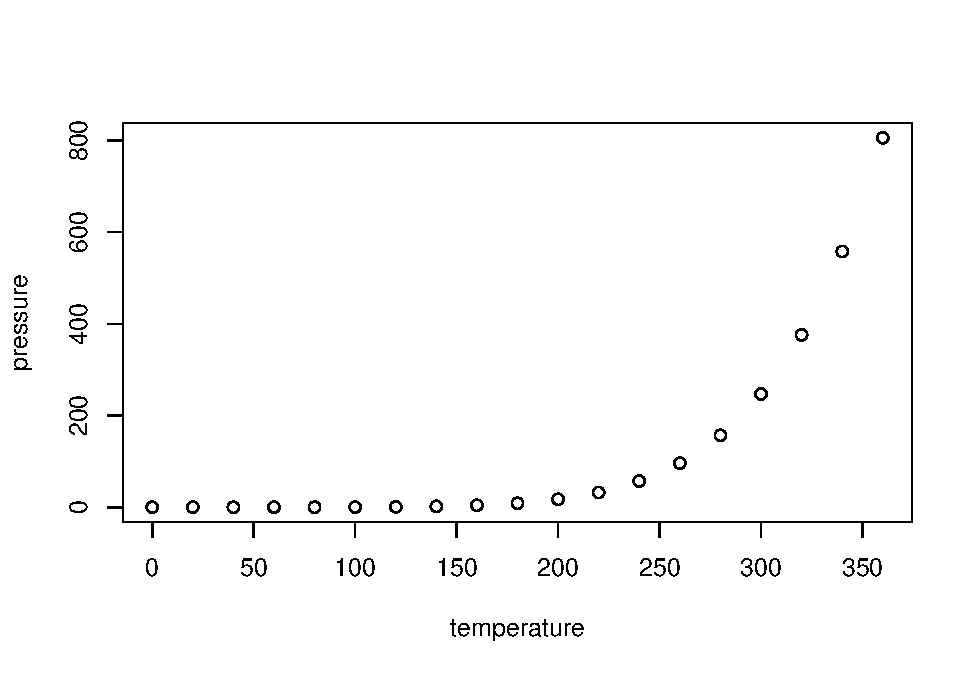
\includegraphics{EconProject_files/figure-latex/pressure-1.pdf}

Note that the \texttt{echo\ =\ FALSE} parameter was added to the code
chunk to prevent printing of the R code that generated the plot.


\end{document}
